\PassOptionsToPackage{dvipsnames,svgnames,table}{xcolor}
\documentclass[11pt]{article}
\usepackage[a4paper,margin=22mm]{geometry}
\usepackage[no-math]{fontspec}
\setmainfont{DejaVu Serif}
\usepackage{amsmath,amssymb,amsthm,mathtools,graphicx,xcolor,hyperref,xurl,xspace,ifthen,enumerate}
\usepackage[shortlabels]{enumitem}
\setlength{\emergencystretch}{4em}
\AtBeginDocument{\special{pdf:mapline pzdr Dingbats <uzdr.pfb}}
\SetMathAlphabet{\mathbf}{normal}{OT1}{cmr}{bx}{n}
\SetMathAlphabet{\mathbf}{bold}{OT1}{cmr}{bx}{n}
\usepackage{thmtools}
\usepackage[capitalize]{cleveref}
\newtheorem{theo}{Theorem}[section]
\newtheorem{lemm}[theo]{Lemma}
\newtheorem{thm}[theo]{Theorem}
\newtheorem{proposition}[theo]{Proposition}
\newtheorem{corollary}[theo]{Corollary}
\newtheorem{definition}[theo]{Definition}
\newtheorem{theorem}[theo]{Theorem}
\newtheorem*{remas*}{Remarks}
\newtheorem{remas}[theo]{Remarks}
\newtheorem*{exam*}{Example}
\newtheorem{ques}[theo]{Question}
\providecommand{\og}{«\nobreakspace}
\providecommand{\fg}{\nobreakspace»}
\newtheorem{lem}[theo]{Lemma}
\newtheorem{lemma}[theo]{Lemma}
\newtheorem{prop}[theo]{Proposition}
\newtheorem{coro}[theo]{Corollary}
\newtheorem{corol}[theo]{Corollary}
\newtheorem*{conj*}{Conjecture}
\newtheorem{conj}[theo]{Conjecture}
\newtheorem{conjecture}[theo]{Conjecture}
\newtheorem{Proposition}[theo]{Proposition}
\newtheorem{theoreme}[theo]{Theorem}
\theoremstyle{definition}
\newtheorem{defi}[theo]{Definition}
\newtheorem{exam}[theo]{Example}
\newtheorem{exem}[theo]{Example}
\newtheorem{remark}[theo]{Remark}
\newtheorem{example}[theo]{Example}
\newtheorem{exams}[theo]{Examples}
\newtheorem{rema}[theo]{Remark}
\newtheorem{nota}[theo]{Notation}
\newtheorem{notation}[theo]{Notation}
\newtheorem*{notas}{Notations}
\newtheorem{result}[theo]{Result}
\newtheorem{question}[theo]{Question}
\newtheorem{prob}[theo]{Problem}
\newtheorem*{rema*}{Remark}
\newtheorem*{defi*}{Definition}
\newtheorem*{theo*}{Theorem}
\newtheorem*{lemm*}{Lemma}
\newtheorem*{prop*}{Proposition}
\newcommand{\enoncename}{}
\newtheorem{corpusenonce}[theo]{\enoncename}
\newenvironment{enonce}[2][]{\renewcommand{\enoncename}{#2}\begin{corpusenonce}}{\end{corpusenonce}}
\newenvironment{enonce*}[2][]{\par\medskip\noindent\textbf{#2.}\itshape}{\par\medskip}
\newenvironment{proofc}[1][\proofname]{\begin{proof}[#1]}{\end{proof}}
\newcommand{\Mc}{\mathcal{M}}
\newcommand{\pointir}{.\ ---\ }
\newcommand{\equalenv}[2]{\expandafter\let\csname#1\expandafter\endcsname\csname#2\endcsname\expandafter\let\csname end#1\expandafter\endcsname\csname end#2\endcsname}
\providecommand{\diagbox}[3][]{\begin{tikzpicture}[x=1em,y=1em,baseline=(current bounding box.center)]\useasboundingbox(0,0) rectangle(3,1.4);\draw(0,1.4)--(3,0);\node at(.5,.3){#2};\node at(2.5,1.1){#3};\end{tikzpicture}}
\providecommand{\eg}{e.g.\ }
\providecommand{\ie}{i.e.\ }
\providecommand{\cf}{cf.\ }
\providecommand{\longthanks}[1]{\par\smallskip\noindent #1\par\smallskip}
\providecommand{\qbinom}[2]{\genfrac{[}{]}{0pt}{}{#1}{#2}}

\providecommand{\mathof}[1]{\mathrm{#1}}

\numberwithin{equation}{section}


\def\endappendix{}


\usepackage{amsmath,amssymb,amsthm,amsfonts}
\usepackage{mathtools}

\usepackage{tikz,graphicx,color}
\usepackage{tikz-cd}
\usepackage{tikz-3dplot}
\usetikzlibrary{calc}
\usetikzlibrary{arrows}
\usetikzlibrary{shapes}
\usetikzlibrary{patterns}
\usetikzlibrary{positioning}
\usetikzlibrary{arrows.meta}
\usetikzlibrary{knots}
\usetikzlibrary{decorations.markings}
\usepackage{epstopdf}

\usepackage[arrow]{xy}

\usepackage{subfig}
\usepackage{arcs}
\usepackage{xcolor}
\usepackage{tabu}
\usepackage{booktabs}

% Unused soul import omitted; no soul text-markup commands occur in retained native body.

\usepackage{letltxmacro}
\usepackage{thmtools,etoolbox}
\usepackage{nameref,hyperref}
\usepackage[capitalize]{cleveref}

\usepackage{tikz-cd}
\usepackage{xspace}

\usepackage{bm}

\newcommand\Acal{\mathcal{A}}\newcommand\Bcal{\mathcal{B}}\newcommand\Ccal{\mathcal{C}}\newcommand\Dcal{\mathcal{D}}\newcommand\Ecal{\mathcal{E}}\newcommand\Fcal{\mathcal{F}}\newcommand\Gcal{\mathcal{G}}\newcommand\Hcal{\mathcal{H}}\newcommand\Ical{\mathcal{I}}\newcommand\Jcal{\mathcal{J}}\newcommand\Kcal{\mathcal{K}}\newcommand\Lcal{\mathcal{L}}\newcommand\Mcal{\mathcal{M}}\newcommand\Ncal{\mathcal{N}}\newcommand\Ocal{\mathcal{O}}\newcommand\Pcal{\mathcal{P}}\newcommand\Qcal{\mathcal{Q}}\newcommand\Rcal{\mathcal{R}}\newcommand\Scal{\mathcal{S}}\newcommand\Tcal{\mathcal{T}}\newcommand\Ucal{\mathcal{U}}\newcommand\Vcal{\mathcal{V}}\newcommand\Wcal{\mathcal{W}}\newcommand\Xcal{\mathcal{X}}\newcommand\Ycal{\mathcal{Y}}\newcommand\Zcal{\mathcal{Z}}

\newcommand\abf{\mathbf{a}}\newcommand\bbf{\mathbf{b}}\newcommand\cbf{\mathbf{c}}\newcommand\dbf{\mathbf{d}}\newcommand\ebf{\mathbf{e}}\newcommand\fbf{\mathbf{f}}\newcommand\gbf{\mathbf{g}}\newcommand\hbf{\mathbf{h}}\newcommand\ibf{\mathbf{i}}\newcommand\jbf{\mathbf{j}}\newcommand\kbf{\mathbf{k}}\newcommand\lbf{\mathbf{l}}\newcommand\mbf{\mathbf{m}}\newcommand\nbf{\mathbf{n}}\newcommand\obf{\mathbf{o}}\newcommand\pbf{\mathbf{p}}\newcommand\qbf{\mathbf{q}}\newcommand\rbf{\mathbf{r}}\newcommand\sbf{\mathbf{s}}\newcommand\tbf{\mathbf{t}}\newcommand\ubf{\mathbf{u}}\newcommand\vbf{\mathbf{v}}\newcommand\wbf{\mathbf{w}}\newcommand\xbf{\mathbf{x}}\newcommand\ybf{\mathbf{y}}\newcommand\zbf{\mathbf{z}}

\newcommand\C{\mathbb{C}}
\newcommand\R{\mathbb{R}}
\newcommand\N{\mathbb{N}}
\newcommand\Z{\mathbb{Z}}
\newcommand\Q{\mathbb{Q}}

\newcommand\Ahat{\hat{A}} 
\newcommand\ipar{{(i)}}
\newcommand\parr[1]{{({#1})}}


\newcommand\m{{\mu}}
\newcommand\lm{{\l/\m}}

\newcommand\Id{\operatorname{Id}}
\newcommand\Vol{\operatorname{Vol}}
\newcommand\diag{{ \operatorname{diag}}}
\newcommand\rank{{ \operatorname{rank}}}
\newcommand\rk{{\mathrm{rank}}}
\newcommand\cork{ \operatorname{corank}}
\newcommand\corank{ \operatorname{corank}}
\newcommand\codim{ \operatorname{codim}}
\newcommand\op{{ \operatorname{op}}}
\newcommand\sh{{ \operatorname{sh}}}
\newcommand\Conv{ \operatorname{Conv}}
\newcommand\Span{ \operatorname{Span}}
\newcommand\proj{ \operatorname{proj}}
\newcommand\sgn{ \operatorname{sgn}}
\newcommand\wt{\operatorname{wt}}
\newcommand\inv{\operatorname{inv}}
\newcommand\Int{\operatorname{int}}
\newcommand\Cone{\operatorname{Cone}}

\newcommand\GL{\operatorname{GL}}
\newcommand\SL{\operatorname{SL}}
\newcommand\Mat{\operatorname{Mat}}
\newcommand\Gr{\operatorname{Gr}}
\newcommand\Grtnn{\Gr_{\ge 0}}
\newcommand\Grtp{\Gr_{>0}}
\newcommand\alt{\operatorname{alt}}
\newcommand\Mattp{\operatorname{Mat}_{>0}}
\newcommand\Mattnn{\operatorname{Mat}_{\ge0}}


\newcommand\Bound{{\rm Bound}}

\newcommand\af{{\rm af}}
\newcommand\Inv{{\rm Inv}}

\newcommand\id{{\operatorname{id}}}

\newcommand\xs{\operatorname{xs}}
\newcommand\ys{\operatorname{ys^{-1}}}
\newcommand\bs{\backslash}
\newcommand\oPi{\accentset{\circ}{\Pi}}
\newcommand\bt{{\mathbf{t}}}
\newcommand\bw{{\mathbf{w}}}
\newcommand\bv{{\mathbf{v}}}
\newcommand\bu{{\mathbf{u}}}
\newcommand\ba{{\mathbf{a}}}
\newcommand\bb{{\mathbf{b}}}
\newcommand\bc{{\mathbf{c}}}
\newcommand\geqJ{\succeq}
\newcommand\gessJ{\succ}

\newcommand\bx{{\bm{x}}}
\newcommand\by{{\bm{y}}}
\newcommand\bi{{\mathbf{i}}}
\newcommand\bj{{\mathbf{j}}}




\newcommand\Deltamp{\Delta^\mp}
\newcommand\Deltapm{\Delta^\pm}


\newcommand\RedMR{\operatorname{Red}}
\newcommand\Red{\operatorname{Red}}
\newcommand\weightL{Y(T)}
\newcommand\rootL{Q_\Phi}
\newcommand\Qkls{Q_P(W,W_J)}


\newcommand\chr{\operatorname{char}}

\let \oldlabel \label
\let\oldref\ref
\let\oldcref\cref





\newcommand\B{{\mathcal B}}
\newcommand\G{\Gcal}
\newcommand\Caff{{\mathcal{C}}}
\newcommand\GCMaff{\tilde{A}}

\newcommand\Phiaff{\Delta}
\newcommand\re{\operatorname{re}}
\newcommand\im{\operatorname{im}}
\newcommand\Phire{\Phiaff_{\re}}
\newcommand\Phiim{\Phiaff_{\im}}

\newcommand\FPS{{\mathcal{A}}}
\newcommand\CRL{{\rootL^\vee}}
\newcommand\minn{{\operatorname{min}}}
\newcommand\Cast{\C^\ast}

\newcommand\tauk{\tau_k}
\newcommand\leqop{\leq^\op}
\newcommand{\Povar}{\mathring{\Pi}}

\newcommand\Boundkn{\operatorname{Bound}(k,\n)}


\newcommand\BAcomb{\psi}
\newcommand\BAgeom{\bar\varphi_u}
\newcommand\BAgeo{\varphi_u}

\newcommand\tht{t}





\newcommand\Ng{{N_g}}
\newcommand\strix{t_1(x)}
\newcommand\strixn{t_1(x_n)}
\newcommand\Bcl{\overline{B}}
\newcommand\epsb{\eps_B}


\newcommand\conept{c}

\newcommand\Link{\operatorname{Lk}}

\newcommand\eps{\varepsilon}






\newcommand\Spec{\operatorname{Spec}}

\newcommand\pr{^{\parr{r}}}

\newcommand\om{\omega}
\newcommand\pan{^\parr{n}}

\newcommand*{\smallcap}{{\mathbin{\scalebox{0.5}{\ensuremath{\cap}}}}}

\newcommand\gc{g_\smallcap}
\newcommand\BG{B_-\backslash G}
\newcommand\BGtnn{(B_-\backslash G)_{\geq0}}

\newcommand\GBsf{(G/B_-)(K)}
\newcommand\BGsf{(\BG)(K)}


\newcommand\str{\operatorname{str}}
\newcommand\strd{\operatorname{str}^\ast}

\newcommand\Sn{S_\n}
\newcommand\chiv{\vec\chi_{v}}

\newcommand\chiw{\vec\chi^{\,w}}
\newcommand\chiww{\vec\chi^{\,{\ww}}}

\newcommand\flec{\vec f}
\newcommand\fR{\vec f}


\newcommand\Ztnn{\Z_{\geq0}}


\newcommand\colspan{\operatorname{ColumnSpan}}

\newcommand\Qkn{Q_{k,\n}}
\newcommand\Bkn{\Boundkn}
\newcommand\Skn{S_\n^{(k)}}

\newcommand\perm{\operatorname{perm}}
\newcommand\Lperm{L^{\perm}}
\newcommand\tor{\operatorname{tor}}
\newcommand\Ltor{L^{\tor}}
\newcommand\grid{\operatorname{grid}}
\newcommand\Lgrid{L^{\grid}}
\newcommand\Lgridt{\tilde L^{\grid}}
\newcommand\rich{\operatorname{Rich}}
\newcommand\Lrich{L^{\rich}}
\newcommand\plab{\operatorname{plab}}
\newcommand\Lplab{L^{\plab}}
\newcommand\cox{\operatorname{Cox}}
\newcommand\Lcox{L^{\cox}}

\newcommand\fp{\pi}


\newcommand\pig{\pi_G}

\newcommand\Arg{\operatorname{arg}}

\newcommand\ice{\operatorname{ice}}
\newcommand\QG{Q_G}
\newcommand\Qice{\widetilde{Q}}
\newcommand\QGice{\Qice_G}

\newcommand\BQ{B(Q)}
\newcommand\BQice{\widetilde{B}(\Qice)}
\newcommand\Vice{\widetilde{V}}

\newcommand\AQ{\Acal(Q)}
\newcommand\AQG{\Acal(\QG)}
\newcommand\AQGice{\Acal(\QGice)}
\def\RQ(#1){R(Q;#1)}
\def\RQX#1#2{R(#1;#2)}
\def\RQice(#1){R(\Qice;#1)}
\def\RQG(#1){R(\QG;#1)}
\newcommand\F{\mathbb{F}}

\newcommand\Pio{\Pi^\circ}
\newcommand\HOMP{P}
\newcommand\unknot{
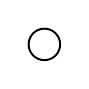
\begin{tikzpicture}[baseline=(ZUZU.base),scale=0.2]\coordinate(ZUZU) at (0,-0.6);
\draw[line width=0.7pt] (0,0) circle (1cm);
  \end{tikzpicture}
}


\newcommand\Top{{\operatorname{top}}}
\def\Ptop_#1(#2){P^\Top(#1;#2)}

\newcommand\fbar{\bar f}
\newcommand\taukn{\tau_{k,\n}}
\newcommand\T{\mathbb{T}}

\newcommand\Cproj{\overline{C}}


\newcommand\fro{\operatorname{fro}}
\newcommand\mut{\operatorname{mut}}
\newcommand\Vfro{V_{\fro}}
\newcommand\Vmut{V_{\mut}}
\newcommand\bip{\operatorname{bip}}
\newcommand\Gbip{G^{\bip}}



\def\Qicefr[#1]{\Qice[#1]}
\newcommand\Bice{\widetilde{B}}
\newcommand\bice{\tilde{B}}
\newcommand\XQice{\Xcal(\Qice)}
\newcommand\XBQice{\Xcal(\BQice)}
\newcommand\AX{\Acal}
\newcommand\AQice{\Acal(\Qice)}
\newcommand\ABQice{\Acal(\BQice)}

\newcommand\chiQ{\chi_Q}
\newcommand\chiQice{\chi_{\Qice}}

\newcommand\Gm{\F^\ast}
\newcommand\Ga{\F}


\newcommand\Aut{\operatorname{Aut}}
\def\QX(#1){Q_{#1}}
\newcommand\disjun{\sqcup}
\newcommand\pmi{\pm I}
\newcommand\pmim{(\pmi)^m}

\newcommand\pmn{\pm I}
\newcommand\pmnm{(\pmn)^m} 
\newcommand\DRW{(\pmn)^m} 

\newcommand\Gbw{G(\bw)}
\def\GX(#1){G(#1)}

\newcommand\rev{\operatorname{rev}}


\newcommand\rowspan{\operatorname{RowSpan}}

\def\figref#1(#2){Figure~\hyperref[#1]{\ref*{#1}(#2)}}

\newcommand\conn{\operatorname{c}}
\newcommand\ncyc{\conn}

\newcommand\n{N}
\newcommand\qq{q^{\frac12}}
\newcommand\qqi{q^{-\frac12}}

\newcommand\disk{\mathbf{D}}

\newcommand\Lrichp{L}

\newcommand\projt{p_{\T}}
\def\projtx#1{\overline{#1}}

\newcommand\Louise{locally acyclic\xspace}
\newcommand\Louiseleaf{recurrent leaf\xspace} 


\newcommand\degtop{\deg^{\Top}}
\newcommand\tI{{\tilde I}}
\newcommand\pmtI{\pm\tI}
\def\linkurl#1{\textup{\texttt{\href{http://katlas.org/wiki/#1}{#1}}}}
\newcommand\comma{} 

\newcommand\Btilde{$\tilde{\text{B}}$}



\def\hopflink{
\scalebox{0.3}{
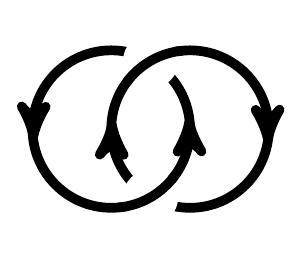
\begin{tikzpicture}[baseline=(ZUZU.base)]\coordinate(ZUZU) at (0,-0.8);
\draw[line width=3.5pt, white,
    decoration={markings,mark=at position 0 with {\arrow[scale=1,black]{stealth'}}},
    decoration={markings,mark=at position 1 with {\arrow[scale=1,black]{stealth'}}},
    postaction={decorate}] (-0.99,-0.15)--(-1,-1)--(1,-1)--(0.99,0.15);
\draw[line width=3.5pt, white,
    decoration={markings,mark=at position 0.01 with {\arrow[scale=1,black]{stealth'}}},
    decoration={markings,mark=at position 0.99 with {\arrow[scale=1,black]{stealth'}}},
    postaction={decorate}] (1.99,-0.15)--(2,-1)--(0,-1)--(0.01,0.15);
\begin{knot}[
    clip width=6,
    flip crossing={1},
    ]
    \strand [line width=3.5pt] (0,0) circle (1.0cm);
    \strand [line width=3.5pt] (1,0) circle (1.0cm);
\end{knot}
\end{tikzpicture} 
}
}

\newcommand\pikn{\pi_{k,\n}}
\newcommand\fkn{f_{k,\n}}


\newcommand\pA{^{(1)}}
\newcommand\pB{^{(2)}}
\newcommand\pC{^{(3)}}
\newcommand\pD{^{(4)}}
\newcommand\pE{^{(5)}}
\newcommand\red{-}
\newcommand\Qred{Q^{\red}}
\newcommand\QredG{Q^{\red}_G}
\newcommand\BQredG{B(\QredG)}

\newcommand\E{H}
\newcommand\Tc{{T,c}}

\newcommand\mysq{
\begin{tikzpicture}
\node[draw=black,line width=1pt, rectangle,scale=0.5,fill=white] (A) at (0,0) {};
\end{tikzpicture}}

\newcommand\tils{\tilde s}


\newcommand\HHH{H\!\!H\!\!H}
\newcommand\HHHC{\HHH_\C}
\newcommand\PGL{\operatorname{PGL}}

\def\mirr#1{#1^\ast}
\newcommand\Divide{\Delta}

\newcommand{\FLY}{HOMFLY\xspace}
\newcommand{\la}{\lambda}
\newcommand{\w}{{\mathbf{w}}}
\newcommand{\pt}{{\rm pt}}
\newcommand{\arxiv}[1]{\href{https://arxiv.org/abs/#1}}



















\begin{document}
\section*{\raggedright 838: Fixed-point-free permutation links agree with reduced plabic and Richardson links, including concave Coxeter realizations}
\noindent\textbf{Author:} Galashin, Pavel; Lam, Thomas\par\noindent\textbf{Source:} Plabic links, quivers, and skein relations. Algebraic Combinatorics 7 (2024), publisher version, DOI 10.5802/alco.345. \url{https://alco.centre-mersenne.org/articles/10.5802/alco.345/}
\par\noindent\textbf{License:} CC BY 4.0, \url{https://creativecommons.org/licenses/by/4.0/}. The original publisher PDF cover has the explicit license notice. See the saved source/license records.
\par\noindent\textbf{Editorial material note (not author text):} The selected problem is Theorem2.5 for the exact fixed-point-free permutation hypothesis: all four authored links are isotopic, and the concave-curve case also realizes the Coxeter link. Full author definitions, Le-diagram/plabic moves and complete planar/toric/strand-by-strand concave winding constructions are retained. The separate quiver/point-count program and later fixed-point sketches are unselected; their pointers keep exact original printed locators. Twenty necessary original diagram-only figures are retained as exact bounded publisher vector assets, with all captions and proof prose/formulas editable native TeX. Only the five original Povar uses in intro context employ a disclosed standard circle-over-capital-Pi typography renderer; body tokens/subscripts remain literal. No isotopy, fixed-point extension, figure or proof has been generated. All proof text and formulas below are editable author TeX. Mathematical wording, language and proof order are retained. Only the article class, title matter and bibliography presentation are adapted for independent compilation; no proof has been generated or repaired.
\par\noindent\textbf{Editorial difficulty:} H2: The author constructs explicit planar, annular and toric isotopies between independently defined links, controlling Le-diagram crossings and strand-by-strand winding in the concave case. Figures 14–18 and the full construction are retained; the fixed-point-free hypothesis avoids the later sketched extension.
\medskip\hrule\medskip
\noindent\textbf{Author statement, complete proof and local supporting text follow in source order.}
\newtheorem{problem}[theo]{Problem}
%\equalenv{example}{exam}
%\equalenv{notation}{nota}

\crefname{figure}{Figure}{Figures}
\crefname{conjecture}{Conjecture}{Conjectures}
%\equalenv{conjecture}{conj}

\addtotheorempostheadhook[theorem]{\crefalias{theoremlisti}{theorem}}
\addtotheorempostheadhook[lemma]{\crefalias{theoremlisti}{lemma}}
\addtotheorempostheadhook[proposition]{\crefalias{theoremlisti}{proposition}}
\addtotheorempostheadhook[corollary]{\crefalias{theoremlisti}{corollary}}

\section{Introduction}
%
%
In recent years, intriguing connections between knot theory and the theory of cluster algebras have been developed.  Shende--Treumann--Williams--Zaslow~\cite{STWZ} suggested the existence of cluster structures for certain moduli spaces of sheaves associated to a Legendrian link, leading to many further developments; see for example \cite{SW,CG,CW}.  Fomin--Pylyavskyy--Shushtin--Thurston~\cite{FPST} studied the relation between quiver mutation and morsifications of algebraic links.  Casals--Gorsky--Gorsky--Simental~\cite{CGGS} and Mellit~\cite{Mellit_Cell} studied braid varieties associated to positive braid words; cluster structures on these spaces are the subject of ongoing works \cite{CGGLSS,GLSBS1,GLSBS2}. Other connections can be found e.g. in~\cite{HiIn,Muller_skein,LeeSch,BMS}.
%

The goal of this work is to compare knot invariants and cluster algebra invariants.  The starting point is our earlier work~\cite{GL_qtcat} on \emph{open positroid varieties} $\Povar_\fp$ \cite{KLS}, which are certain distinguished subvarieties of the Grassmannian equipped with a cluster structure \cite{GL_cluster} (see also~\cite{Scott,MSLA,Lec,SSBW}).  In \cite{GL_qtcat}, we associated a \emph{positroid link} $L_\fp$ to each open positroid variety $\Povar_\fp$, and constructed an isomorphism between the cohomology of $\Povar_\fp$ and the top $a$-degree part of the Khovanov--Rozansky triply-graded link homology~\cite{KR1,KR2,KhoSoe} of $L_\fp$.   In subsequent work~\cite{GL_cat_combin}, we further developed this connection by defining \emph{positroid Catalan numbers} as certain Euler characteristics of open positroid varieties.  This invariant was studied for a subclass of permutations arising from concave curves, using a Dyck path recursion that did not require explicit mention of the cluster structure on $\Povar_\fp$, or of the positroid link $L_\fp$.

The initial motivation of this work is to explain our positroid recursion in the broader setting of \emph{plabic (i.e. planar bicolored) graphs}, making an explicit connection to recursions for quivers and for links.  Plabic graphs were introduced by Postnikov~\cite{Pos} who also speculated on the relation with cluster algebras. 
%
%
 To an arbitrary plabic graph $G$ one can associate a \emph{plabic graph link} $\Lplab_G$ introduced in~\cite{FPST,STWZ}.
 %
 On the other hand, the set of equivalence classes of \emph{reduced} plabic graphs is in bijection with open positroid varieties, to which we associated positroid links in~\cite{GL_qtcat}.

In the first part of this work, we establish (\cref{thm:isotopy}) that the various links associated to $\Povar_\fp$ are isotopic, including the positroid link $L_\fp$ and the corresponding plabic graph link $\Lplab_G$.  In the second part of this work, we study the relation between the point count function of a quiver $Q$ and the HOMFLY polynomial $\HOMP(L;a,z)$ of a link.  We introduce a class of \emph{simple} plabic graphs. Our main conjecture (Conjecture~2.8) states that for a simple plabic graph $G$, the point count of the planar dual quiver $Q_G$ is equal to the top $a$-degree part of the HOMFLY polynomial of $\Lplab_G$.  We show (Theorem~2.9) that this conjecture holds for the class of \emph{leaf recurrent} plabic graphs, that includes reduced plabic graphs and plabic fences. 
We interpret and generalize the locally acyclic\footnote{We call a quiver \Louise if it satisfies the ``Louise condition" of~\cite{MSLA,LS}.  This is stronger than the notion of local acyclicity used in \cite{Muller}.} recursion for positroids~\cite{MSLA} in terms of the \FLY skein relation.
%
 %
 
\section{Main results}
Let $\fp\in\Sn$ be a permutation. For simplicity (cf. Section~4.5), we assume that $\fp$ has no fixed points, i.e.  $\fp(i)\neq i$ for all $i\in[\n]:=\{1,2,\dots,\n\}$. 
 %

\begin{figure}
\begin{tabular}{cccc}
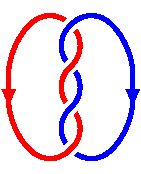
\includegraphics[width=0.13\textwidth]{../assets/838/L4a1.pdf} &
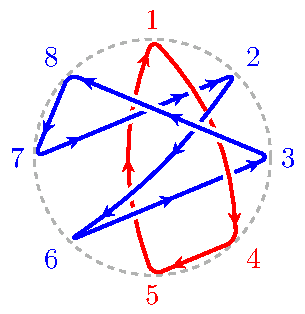
\includegraphics[width=0.27\textwidth]{../assets/838/Lperm.pdf} &
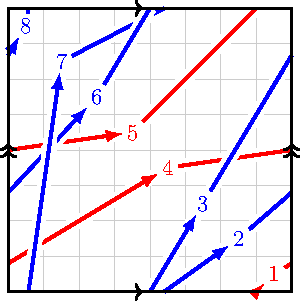
\includegraphics[width=0.24\textwidth]{../assets/838/Ltor.pdf}&
\hspace{0.05in}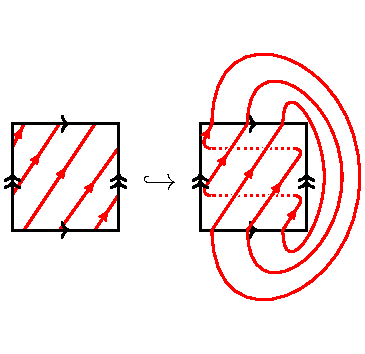
\includegraphics[width=0.25\textwidth]{../assets/838/Ltor_emb.pdf}\\
  (a) \linkurl{L4a1} & (b) $\Lperm_\pi$ & (c) $\Ltor_\pi$ & (d) \hspace{0.05in}$\T\hookrightarrow\R^3$
\end{tabular}
%
%
%
%
%
%
  \caption{\label{fig:L4a1} The links \linkurl{L4a1}$\cong \Lperm_\pi\cong\Ltor_\pi$ for $\pi$ given by~\eqref{eq:intro:fp}.}
\end{figure}


In~\cite{GL_qtcat}, we described a way to associate a \emph{positroid link} $L_\fp$ to such $\fp$. The number of components of $L_\fp$ is given by the number $\ncyc(\fp)$ of cycles of $\fp$. Our running example will be
\begin{equation}\label{eq:intro:fp}
 \fp=\left(\!\!\text{
\begin{tabular}{cccccccc}
\textcolor{red}{$1$} & \textcolor{blue}{$2$} & \textcolor{blue}{$3$} & \textcolor{red}{$4$} & \textcolor{red}{$5$} & \textcolor{blue}{$6$} & \textcolor{blue}{$7$} & \textcolor{blue}{$8$}\\
\textcolor{red}{$4$} & \textcolor{blue}{$6$} & \textcolor{blue}{$8$} & \textcolor{red}{$5$} & \textcolor{red}{$1$} & \textcolor{blue}{$3$} & \textcolor{blue}{$2$} & \textcolor{blue}{$7$}
\end{tabular}
}\!\!\right),
\end{equation}
written in two-line notation, with different colors representing different cycles of $\fp$. We have $\n=8$ and $\ncyc(\fp)=2$. The associated positroid link $L_\fp$ is shown in \figref{fig:L4a1}(a); it appears under the name \linkurl{L4a1} in the Thistlethwaite Link Table~\cite{KAT}. 

\subsection{Positroid links} \label{sec:intro:positroid_links}

Our first result relates several different representations of the link $L_\fp$, confirming the conjectures of~\cite{GL_qtcat,GL_cat_combin}. We start by giving a brief overview of these descriptions; see \cref{sec:positr-comb,sec:positr-link-isot} for full details.

\subsubsection{Permutation link} \label{sec:intro:perm_links}
Draw $\n$ points labeled $1,2,\dots,\n$ on the circle in clockwise order. Draw a line segment connecting $i$ to $\fp(i)$, for each $i\in[\n]:=\{1,2,\dots,\n\}$. If two line segments $[i, \fp(i)]$, $[j,\fp(j)]$ cross for some $i,j\in[\n]$ such that $\fp(i)<\fp(j)$, then the segment $[j,\fp(j)]$ is drawn above $[i, \fp(i)]$; see \figref{fig:L4a1}(b). 
%
 The union of these segments gives rise to a link diagram. We refer to the resulting link as the \emph{permutation link} of $\fp$, denoted $\Lperm_\fp$. Orienting each line segment from $i$ to $\fp(i)$ induces an orientation on $\Lperm_\fp$.


\subsubsection{Toric permutation link}\label{sec:intro:tor_links} Let $\T:=\R^2/\Z^2$ be the torus. Consider its fundamental domain $[0,1]^2$ which we view as a square subdivided into $\n^2$ boxes of size $\frac1\n\times \frac1\n$. We denote by $b_{i,j}$, $1\leq i,j\leq \n$, the box whose upper right corner has coordinates $\frac1\n(i,j)$. For each $i\in[\n]$, place a dot $d_i$ in box $b_{i,\n+1-i}$. Draw an arrow (in $\T$) in the northeast direction from $d_i$ to $d_{\fp(i)}$ for each $i\in[\n]$. When two such arrows cross, the arrow with the higher slope is drawn above the arrow with the lower slope. We obtain a planar diagram of an oriented link $\Ltor_\fp$ drawn on the surface of $\T$; see \figref{fig:L4a1}(c). Any link drawn on $\T$ may be converted into a link in $\R^3$ using the procedure shown in \figref{fig:L4a1}(d). Abusing notation, we denote by $\Ltor_\fp$ the resulting link in $\R^3$.

\begin{remark}
Viewing $\Ltor_\fp$ as drawn on the surface of $\T$ (resp. in a solid torus $S^1\times [0,1]^2$) contains more information---it gives rise to a certain elliptic Hall algebra element~\cite{ScVa,BuSc} (resp. to a symmetric 
%
function~\cite{Turaev}) with deep connections to Khovanov--Rozansky homology. We aim to pursue this direction in an upcoming paper~\cite{GL_EHA}.
\end{remark}
%
%


\begin{figure}
  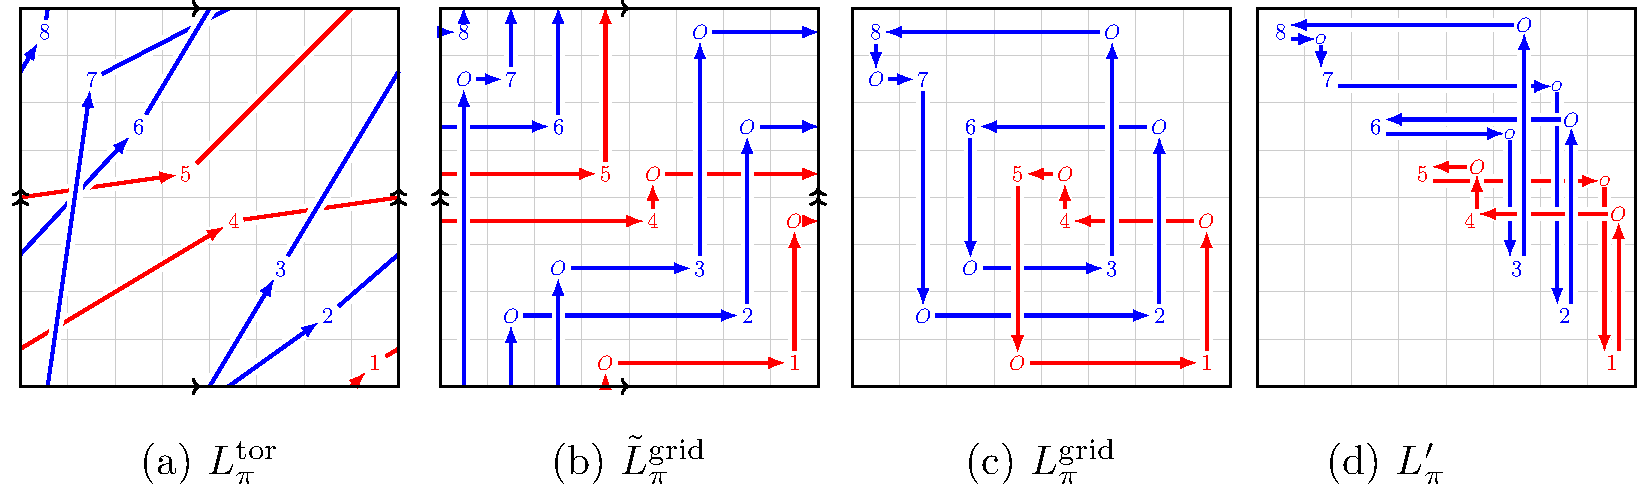
\includegraphics[width=1.0\textwidth]{../assets/838/grid_iso.pdf}
  %
 \caption{\label{fig:grid_iso} Toric grid links; see \cref{rmk:grid} and \cref{sec:perm-to-toric}.}
\end{figure}


\begin{remark}\label{rmk:grid}
We may also view $\Ltor_\fp$ as coming from a \emph{grid diagram} (see e.g.~\cite{OSS}). The grid diagram of $\fp$ is obtained by placing an $X$ in box $b_{i,\n+1-i}$ and an $O$ in box $b_{i,\n+1-\fp(i)}$ for each $i\in[\n]$. We then connect the $X$'s and the $O$'s by horizontal and vertical segments, always drawing the vertical segments above the horizontal ones. More precisely, to a given grid diagram, we can associate two links. First, a \emph{toric grid link} $\Lgridt_\pi$, drawn on the surface of $\T$, is obtained by drawing a horizontal arrow from $O$ to $X$ pointing right in each row, and a vertical arrow from $X$ to $O$ pointing up in each column; see \figref{fig:grid_iso}(b). (In \cref{fig:grid_iso}, for each $i\in[\n]$, we place an $i$ instead of an $X$ in box $b_{i,\n+1-i}$.) Second, a \emph{planar grid link} $\Lgrid_\pi$, whose planar diagram is drawn inside $[0,1]^2$, is obtained by drawing a horizontal arrow from $O$ to $X$ in each row, and a vertical arrow from $X$ to $O$ in each column, but in this case the arrows are not allowed to cross the boundaries of $[0,1]^2$; see \figref{fig:grid_iso}(c). As explained in~\cite[Section~3.2]{OSS}, these two links are isotopic to each other. It is easy to see that the toric grid link $\Lgridt_\pi$ is also isotopic to $\Ltor_\fp$.
\end{remark}

%


\begin{figure}
  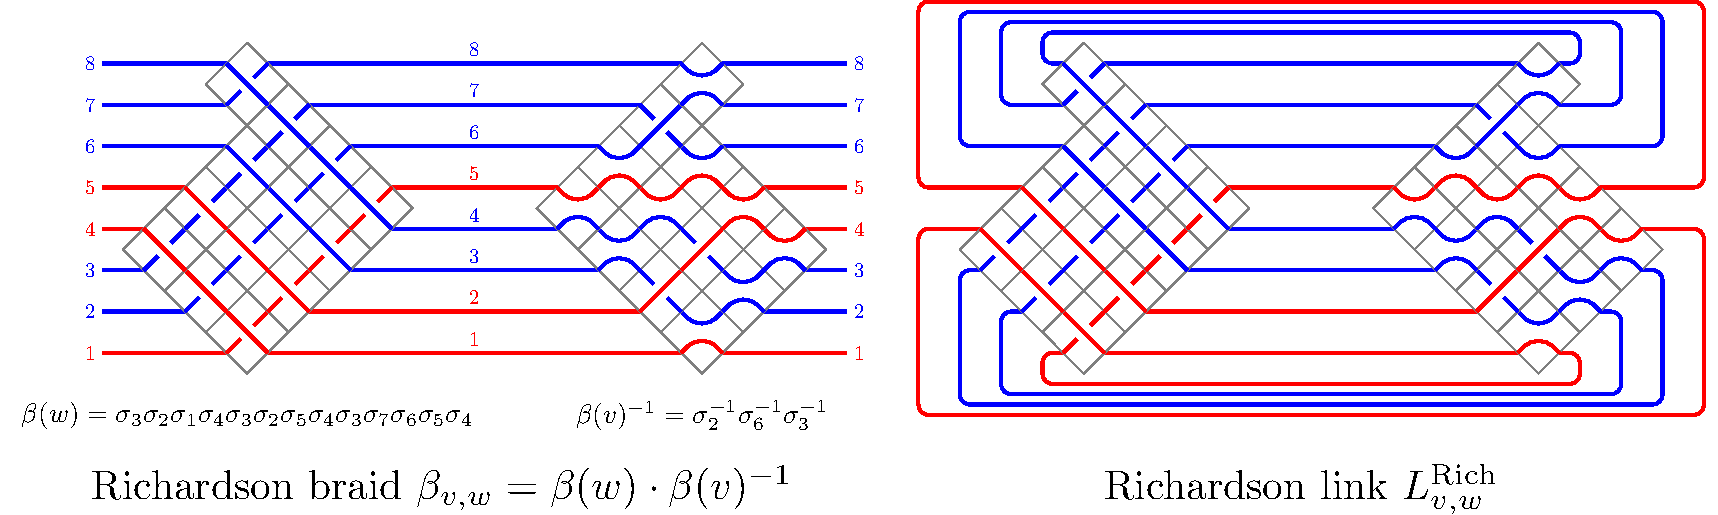
\includegraphics[width=1.0\textwidth]{../assets/838/Lrich.pdf}
  \caption{\label{fig:Lrich} A Richardson braid (left) and a Richardson link (right) defined in \cref{sec:intro:Rich_link}.}
\end{figure}


\subsubsection{Richardson link}\label{sec:intro:Rich_link} A permutation $w\in\Sn$ is called \emph{$k$-Grassmannian} if $w(1)<\cdots<w(\n-k)$ and $w(\n-k+1)<\cdots<w(\n)$. We denote by $\Skn$ the set of $k$-Grassmannian permutations. The permutation $\fp$ can be uniquely decomposed as the product $\fp=wv^{-1}$ for some $1\leq k\leq \n-1$ and some pair $(v,w)\in \Sn\times\Skn$ such that $v\leq w$ in the Bruhat order on~$\Sn$; see \cref{cor:KLS}. For the permutation $\fp$ given by~\eqref{eq:intro:fp}, we get that $k=4$ and\footnote{Our convention for multiplying permutations is right-to-left, i.e.  $\fp(j)=w(v^{-1}(j))$ for all $j\in[\n]$.}
\begin{equation*}%
v=\left(\!\!\text{
\begin{tabular}{cccccccc}
\textcolor{red}{$1$} & \textcolor{red}{$2$} & \textcolor{blue}{$3$} & \textcolor{blue}{$4$} & \textcolor{red}{$5$} & \textcolor{blue}{$6$} & \textcolor{blue}{$7$} & \textcolor{blue}{$8$}\\
\textcolor{red}{$1$} & \textcolor{red}{$4$} & \textcolor{blue}{$2$} & \textcolor{blue}{$3$} & \textcolor{red}{$5$} & \textcolor{blue}{$7$} & \textcolor{blue}{$6$} & \textcolor{blue}{$8$}
\end{tabular}
}\!\!\right)
,\quad
w=\left(\!\!\text{
\begin{tabular}{cccccccc}
\textcolor{red}{$1$} & \textcolor{red}{$2$} & \textcolor{blue}{$3$} & \textcolor{blue}{$4$} & \textcolor{red}{$5$} & \textcolor{blue}{$6$} & \textcolor{blue}{$7$} & \textcolor{blue}{$8$}\\
\textcolor{red}{$4$} & \textcolor{red}{$5$} & \textcolor{blue}{$6$} & \textcolor{blue}{$8$} & \textcolor{red}{$1$} & \textcolor{blue}{$2$} & \textcolor{blue}{$3$} & \textcolor{blue}{$7$}
\end{tabular}
}\!\!\right)
.
\end{equation*}
%
Here, the colors represent the cycles of $\fp=wv^{-1}$. 
 Let $\beta(v),\beta(w)$ be the positive braid lifts of $v,w$ to the braid group of $\Sn$. Consider the \emph{Richardson braid} $\beta_{v,w}:=\beta(w)\cdot \beta(v)^{-1}$ shown in \figref{fig:Lrich}(left). Taking the \emph{braid closure} of $\beta_{v,w}$, we obtain the \emph{Richardson link} $\Lrich_{v,w}=\Lrich_\fp$ shown in \figref{fig:Lrich}(right). We orient the strands of $\beta_{v,w}$ from right to left; cf. \figref{fig:Lrich-to-L'}(left).
%
\begin{remark}\label{rmk:Rich_Young}
It is well known (cf. \cref{sec:Le-diags}) that $k$-Grassmannian permutations are in bijection with Young diagrams that fit inside a $k\times (\n-k)$ rectangle. Thus, in \figref{fig:Lrich}(left), we arrange the crossings in $\beta(w)$ into a (rotated) Young diagram. The condition that $v\leq w$ in the Bruhat order implies that a reduced word for $v$ is a subword of a reduced word for $w$, and thus we represent $\beta(v)^{-1}$ in \figref{fig:Lrich}(left) by replacing some of the crossings in $\beta(w)^{-1}$ with ``elbows.''
%
\end{remark}

 The above recipe was used in~\cite{GL_qtcat} more generally for pairs $v\leq w$ where $w$ is not necessarily $k$-Grassmannian. 

\begin{figure}
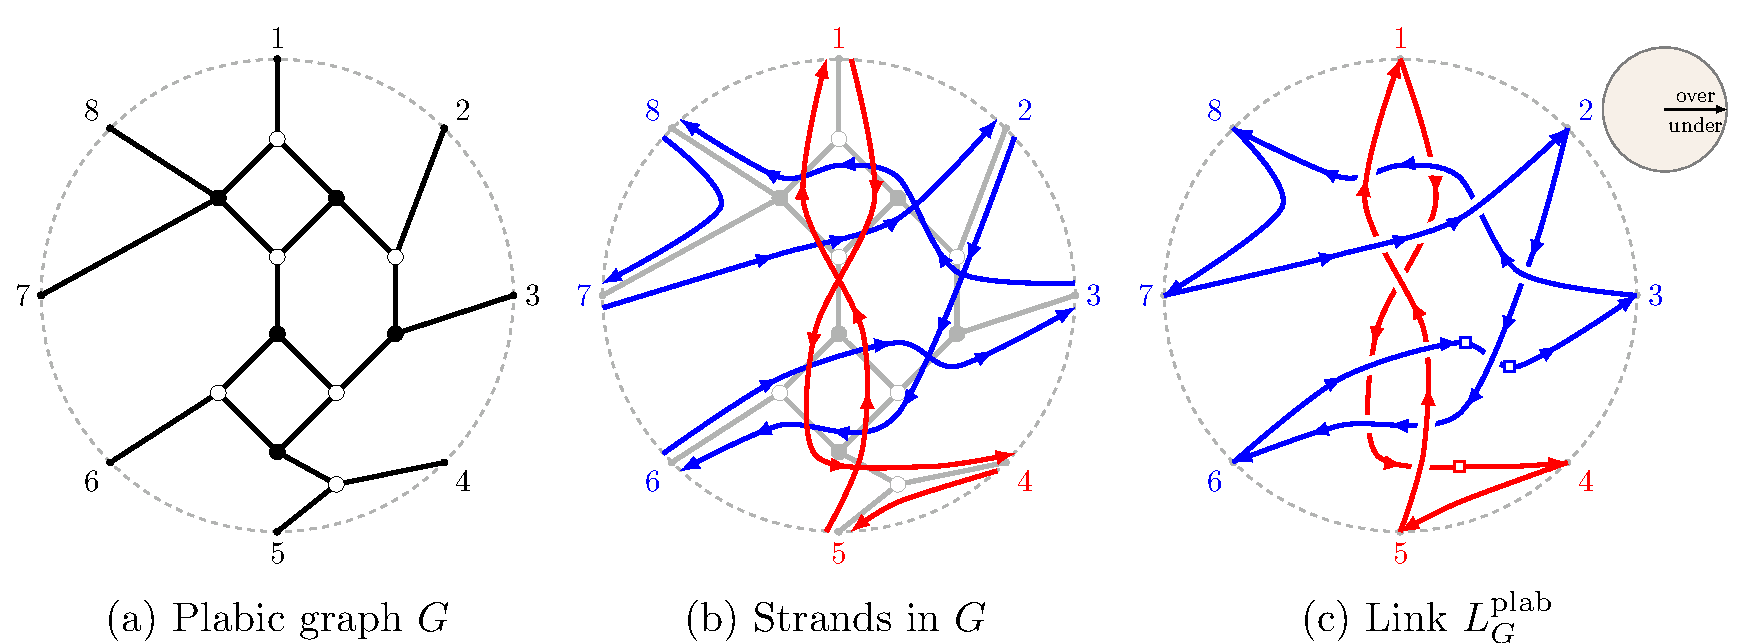
\includegraphics[width=1.0\textwidth]{../assets/838/Lplab.pdf}
  \caption{\label{fig:Lplab} Converting a plabic graph $G$ into the plabic graph link $\Lplab_G$.}
\end{figure}


\subsubsection{Plabic link} \label{sec:intro:plabic_link}
%
A \emph{plabic graph} is a non-empty planar graph $G$ embedded in a disk with vertices colored black and white; see~\cite{Pos}.  
%
 A \emph{strand} in $G$ is a path that makes a sharp right turn at each black vertex and a sharp left turn at each white vertex. We assume that the graph $G$ has $\n$ boundary vertices, all of which have degree $1$ and are labeled $1,2,\dots,\n$ in clockwise order. An example of a plabic graph $G$ is shown in \figref{fig:Lplab}(a), and the strands in $G$ are shown in \figref{fig:Lplab}(b).

The following description of the \emph{plabic graph link} $\Lplab_G$, or \emph{plabic link} for short, can be deduced from~\cite{ACampo,STWZ,FPST} by breaking the symmetry following~\cite{Hirasawa}. (See \cref{sec:plabic_links_properties} for a more invariant description.) The planar diagram of $\Lplab_G$ will consist of the union of the strands of $G$. To specify the overcrossings, let $p$ be an intersection point of two strands $S_1,S_2$ in $G$.  The tangent vector to $S_1$ (resp. $S_2$) at $p$ can be considered a vector in the complex plane, and we let $\Arg(S_1,p) \in[0,2\pi)$ (resp. $\Arg(S_2,p)\in[0,2\pi)$) denote the argument of this vector.
%
We assume that $0<\Arg(S_1,p)\neq\Arg(S_2,p)<2\pi$. Then $S_1$ is drawn above $S_2$ if $\Arg(S_2,p)>\Arg(S_1,p)$, otherwise $S_1$ is drawn below $S_2$. 

\begin{figure}
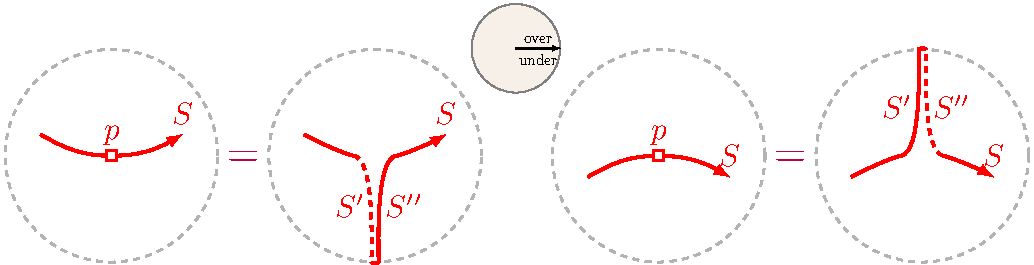
\includegraphics[width=0.7\textwidth]{../assets/838/over_under.pdf}
  \caption{\label{fig:over_under} For every point $p$ on a strand $S$ satisfying $\Arg(S,p)=0$, we insert a strand segment going to the boundary and back; see \cref{sec:intro:plabic_link}.}
\end{figure}



A technical extra step is required to finalize the construction of $\Lplab_G$; see \cref{fig:over_under}. Consider a point $p$ on a strand $S$ such that $\Arg(S,p)=0$, i.e.  such that $S$ is directed to the right at $p$. We add an extra segment $S'$ to $S$ traveling from $p$ to the boundary of the disk followed by a segment $S''$ traveling from the boundary back to $p$. In the neighborhood of $p$, $S$ looks like a plot of a function. If this function is ``concave up'' at $p$ (i.e.  has positive second derivative), then $S'$ (resp. $S''$) is drawn below (resp. above) all other strands. If $S$ is ``concave down'' at $p$ then $S'$ (resp. $S''$) is drawn above (resp. below) all other strands. 

Finally, each boundary vertex of $G$ is an endpoint of exactly two strands (one outgoing and one incoming). We join these endpoints together and obtain a planar diagram of a link denoted $\Lplab_G$. See \figref{fig:Lplab}(c), where the points $p$ such that $\Arg(S,p)=0$ are marked by the symbol $\mysq$.

 The strands in $G$ that start and end at the boundary vertices give rise to the \emph{strand permutation} $\pig$ of $G$. In this subsection, we will assume that $G$ is \emph{reduced}, i.e.  that $G$ has the minimal possible number of faces among all graphs with a given strand permutation. Importantly, in Section~2.2, we will drop this assumption. Postnikov~\cite{Pos} showed that for any $\pi\in \Sn$, there exists a reduced plabic graph $G$ with strand permutation $\pig=\pi$. For example, for $\pi$ given by~\eqref{eq:intro:fp}, one can take $G$ to be the graph in \figref{fig:Lplab}(a). Up to isotopy, the resulting link $\Lplab_G$ depends only on $\pi$ and is denoted $\Lplab_\pi$. 

%
%
%

%


%
%


\begin{figure}
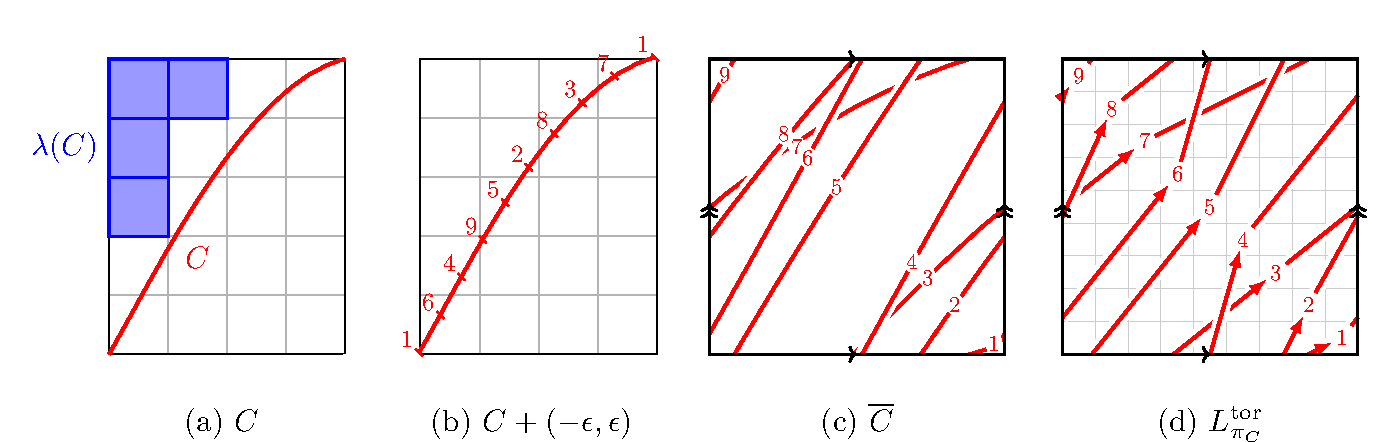
\includegraphics[width=1.0\textwidth]{../assets/838/concave_1.pdf}
  \caption{\label{fig:concave} Converting a concave curve $C$ into the link $\Ltor_{\pi_C}$ for some $\pi_C\in\Sn$; see \cref{ex:intro:Cox}.}
\end{figure}


\subsubsection{Coxeter link} \label{sec:intro:cox_link}
In~\cite[Section~6]{GL_cat_combin}, we studied \emph{concave permutations}, defined as follows. Choose a generic concave curve $C$ inside a $k\times (\n-k)$ rectangle connecting $(0,0)$ to $(\n-k,k)$ as in \figref{fig:concave}(a). We will shift it by the vector $(-\eps,\eps)$ for some small $\eps>0$ as in \figref{fig:concave}(b). Under the natural projection $\R^2\to\T=\R^2/\Z^2$, the curve $C+(-\eps,\eps)$ projects to a curve $\Cproj$ in the unit square $[0,1]^2$. For each self-intersection of $\Cproj$, we draw the segment of the higher slope above the segment of the lower slope; see \figref{fig:concave}(c). The resulting link diagram is isotopic to $\Ltor_\pi$ for a permutation $\pi=\pi_C\in\Sn$ which can be explicitly read off from $\Cproj$ as follows. Label the intersection points of $\Cproj$ with the $y=1-x$ diagonal of $[0,1]^2$ by $d_1,d_2,\dots,d_\n$, proceeding in the northwest direction. Thus, $d_1=(1-\eps,\eps)$ is the projection of the starting and ending points of $C+(-\eps,\eps)$. In \figref{fig:concave}(c), we represent each point $d_i$ by~$i$. Since $C$ was generic, we assume that the points $d_1,d_2,\dots, d_\n$ are pairwise distinct. The permutation $\pi_C$ is defined so that each segment of $C$ connects (in the northeast direction) $d_i$ to $d_{\pi(i)}$ for some $i\in[\n]$. See \figref{fig:concave}(d). We refer to permutations that can be obtained in this way as \emph{concave permutations}. They form a subclass of the class of \emph{repetition-free permutations} introduced in~\cite{GL_cat_combin}.

Let $\la_C=(\la_1,\la_2,\dots,\la_k)$ be the Young diagram inside the $k\times (\n-k)$ rectangle consisting of all unit boxes strictly above $C$, shown in \figref{fig:concave}(a). 
%
 Consider a sequence $\abf(C)=(a_2,\dots,a_k)$ given by $a_i:=\la_{i-1}-\la_i$ for $2\leq i\leq k$. The \emph{Coxeter link} $\Lcox_C$ is the closure of the braid
\begin{equation}\label{eq:beta_abf_dfn}
  \beta(\abf(C)):=\ell_2^{a_2}\cdots \ell_k^{a_k}\cdot\sigma_1\cdots \sigma_{k-1},
\end{equation}
where $\sigma_1,\dots,\sigma_{k-1}$ are the standard braid group generators of the braid group of $S_k$, and $\ell_i=\sigma_{i-1}\cdots \sigma_1\cdot \sigma_1\cdots \sigma_{i-1}$ are the Jucys--Murphy elements. 

\begin{figure}
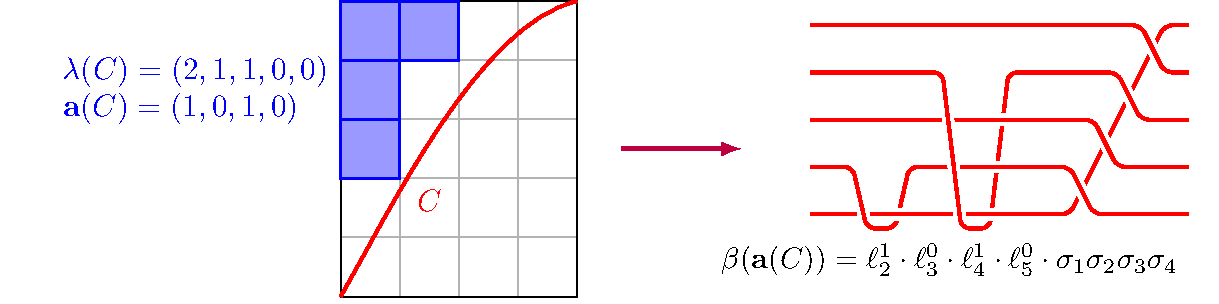
\includegraphics[width=0.85\textwidth]{../assets/838/concave_2.pdf}
  \caption{\label{fig:concave_2} Converting a concave curve $C$ into the Coxeter braid $\beta(\abf(C))$.}
\end{figure}
\begin{example}\label{ex:intro:Cox}
Let $C$ be the curve shown in \cref{fig:concave,fig:concave_2}. We have $k=5$ and $\n=9$. The permutation $\pi_C=\left(\!\!\text{
\begin{tabular}{ccccccccc}
%
%
$1$ & $2$ & $3$ & $4$ & $5$ & $6$ & $7$ & $8$ & $9$\\
$6$ & $8$ & $7$ & $9$ & $2$ & $4$ & $1$ & $3$ & $5$
\end{tabular}
}\!\!\right)$ can be read off from the labels\footnote{The labels in \figref{fig:concave}(b) are chosen in such a way that when we project $C$ to the unit square, they become ordered along the diagonal $y=1-x$; see \figref{fig:concave}(c).} in \figref{fig:concave}(b): in cycle notation, $\pi_C$ is given by $\pi_C=(1\,6\,4\,9\,5\,2\,8\,3\,7\,1)$. We have $\la_C=(2,1,1,0,0)$, $\abf(C)=(1,0,1,0)$,  and $\beta(\abf(C))=\ell_2\ell_4\sigma_1\sigma_2\sigma_3\sigma_4$; see also~\cite[Figure~13]{GL_cat_combin}.
\end{example}
%
 Coxeter links and their Khovanov--Rozansky homology have previously been studied in relation to flag Hilbert schemes and generalized shuffle conjectures~\cite{ObRo,GN,GNR,BHMPS}; see also~\cite[Section~7.2]{GL_cat_combin}.
%
 %
%
%

The following is our first main result.
\begin{theorem}\label{thm:isotopy}
  Let $\fp\in\Sn$ be a permutation without fixed points. Then the links $\Lperm_\fp$, $\Ltor_\fp$, $\Lrich_\fp$, and $\Lplab_\fp$ are all isotopic. If $\fp=\fp_C$ for some concave curve $C$ then each of these links is also isotopic to $\Lcox_C$.
%
\end{theorem}
We refer to any one of the above links as the \emph{positroid link} of $\fp$.

%
%
%

%

%


\begin{remark}
The recent work~\cite{CGGS} independently constructs Legendrian isotopies (a stronger result than our smooth isotopies) between the Richardson link $\Lrich_\pi$ and other closely related links: closures of juggling braids, cyclic rank matrix braids, and Le-diagram braids.  We expect the Le-diagram braid in~\cite{CGGS} to be closely related to our plabic graph link $\Lplab_\fp$, and the juggling braid to be similar to our permutation link $\Lperm_\fp$, though we believe our definition of $\Lperm_\fp$ is the simplest and most elementary.

Isotopies between cyclic rank matrix links and plabic graph links have also been observed in~\cite{STWZ}.
%
%
\end{remark}

\section{Positroid combinatorics}\label{sec:positr-comb}
In this section, we review some background on the combinatorics of plabic graphs and the associated objects.


\subsection{Bounded affine permutations}\label{sec:bound-affine-perm}
A \emph{$(k,\n)$-bounded affine permutation}~\cite{KLS} is a bijection $f:\Z\to\Z$ such that 
\begin{itemize}
\item $f$ is \emph{$\n$-periodic}: $f(i+\n)=f(i)+\n$ for all $i\in \Z$,
\item  $i\leq f(i)\leq i+\n$ for all $i\in\Z$, and %
\item $\sum_{i=1}^\n(f(i)-i)=k\n$.
\end{itemize}
The set of $(k,\n)$-bounded affine permutations is denoted $\Boundkn$. Each $f\in\Boundkn$ gives rise to a unique permutation $\fbar\in\Sn$ defined by $\fbar(i)\equiv f(i)\pmod \n$ for each $i\in[\n]$. Given $f\in\Boundkn$, an integer $i\in\Z$ is called a \emph{loop} (resp. a \emph{coloop}) of $f$ if $f(i)=i$ (resp. $f(i)=i+\n$). Thus, $\fbar$ has no fixed points if and only if $f$ has no loops and no coloops. In this case, $f$ is uniquely determined by $\fbar$, and the integer $k$ is recovered from $\fbar$ as follows:
\begin{equation*}%
  k=k(\fbar):=\#\{i\in[\n]\mid \fbar(i)<i\}.
\end{equation*}
We define $\taukn\in\Boundkn$  by
\begin{equation*}%
  \taukn(i)=
  \begin{cases}
    i, &\text{if $1\leq i\leq \n-k$,}\\
    i+\n, &\text{if $\n-k+1\leq i\leq \n$,}
  \end{cases}
\end{equation*}
and extend it to a function $\taukn:\Z\to\Z$ by $\n$-periodicity. 


Let $\Qkn:=\{(v,w)\in \Sn\times \Skn\mid v\leq w\}$, where $\leq$ denotes the Bruhat order on $\Sn$. Given a permutation $u\in\Sn$, we can extend it to an $\n$-periodic map $\tilde u:\Z\to\Z$ defined by $\tilde u(i)=u(i)$ for $i\in[\n]$. For $(v,w)\in\Qkn$, let $f_{v,w}:=\tilde w\taukn\tilde v^{-1}$. By~\cite[Proposition~3.15]{KLS}, the map $(v,w)\mapsto f_{v,w}$ gives a bijection $\Qkn\xrightarrow{\sim} \Boundkn$. Taking the inverse of this map, we obtain the following result, justifying the definition of a Richardson link in \cref{sec:intro:Rich_link}.
\begin{corollary}\label{cor:KLS}
If $\fp\in\Sn$ has no fixed points then it can be uniquely factored as a product $\fp=wv^{-1}$, where $(v,w)\in\Qkn$ and $k=k(\fp)$.
\end{corollary}

The open positroid stratification~\cite{KLS} of the Grassmannian contains a unique open dense stratum. It is labeled by the bounded affine permutation $\fkn\in\Boundkn$ sending $i\mapsto i+k$ for all $i\in\Z$. We let $\pikn\in\Sn$ be the permutation sending $i\mapsto i+k$ modulo $\n$ for all $i\in[\n]$.


\subsection{Plabic graphs}\label{sec:plabic-graphs}
%
%
%
%
%
%
%
%
%
%
%

\begin{figure}
  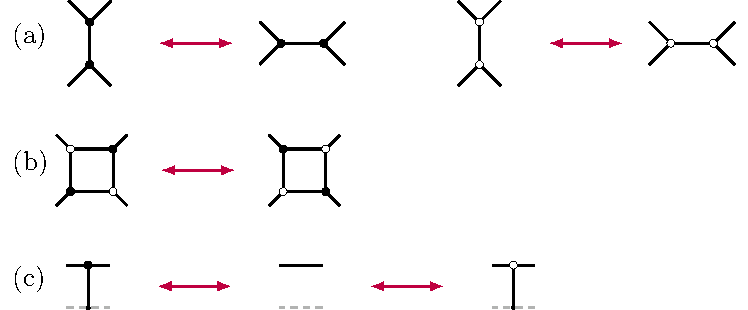
\includegraphics[width=0.7\textwidth]{../assets/838/moves.pdf}
  \caption{\label{fig:moves} Local moves for plabic graphs: (a) contraction-uncontraction move; (b) square move; (c) tail addition/removal.}
\end{figure}




%

%

Let $G$ be a plabic graph. Recall from \cref{sec:intro:plabic_link} that $G$ must be nonempty, that the boundary vertices of $G$ are labeled by $1,2,\dots,\n$ in clockwise order, and that the strand permutation $\pig:[\n]\to[\n]$ sends $i\mapsto j$ whenever the strand starting at $i$ terminates at $j$. We always assume that our plabic graphs $G$ are such that $\pig$ has no fixed points, although most of our constructions can be easily extended to this case; see Section~4.5.

%

\begin{definition}[\cite{Pos}]
We say that $G$ is \emph{reduced} if it has the minimal number of faces among all plabic graphs with strand permutation $\pig$.
\end{definition}
Alternatively~\cite[Theorem~13.2]{Pos}, a plabic graph $G$ is reduced if and only if $G$ has no closed strands, no self-intersecting strands, and no pairs of strands forming a \emph{bad double crossing} shown in \figref{fig:double}(right). \emph{Good double crossings} shown in \figref{fig:double}(left) are allowed.

We consider several types of \emph{local moves} on plabic graphs, shown in \cref{fig:moves}. 
%
 It was shown in~\cite{Pos} that every permutation $\pi\in\Sn$ is the strand permutation of some reduced plabic graph $G$, and that moreover, any two reduced plabic graphs with the same strand permutation are related by a sequence of the moves (a) and (b) in \cref{fig:moves}. Below we review one construction of plabic graphs which will be particularly useful to us.

\subsection{Le-diagrams}\label{sec:Le-diags}
Let $\la=(\la_1\geq\la_2\geq\cdots\geq\la_k\geq0)$ be a partition, which we identify with its Young diagram. We assume that this Young diagram fits inside a $k\times (\n-k)$ rectangle, i.e.  satisfies $\la_1\leq \n-k$. We draw Young diagrams using \emph{English} (or \emph{matrix}) \emph{notation}. We use matrix coordinates for the boxes of $\la$, thus, row $i$ contains boxes with coordinates $(i,j)$ for $1\leq j\leq \la_i$, and box $(1,1)$ is the top left box.

A \emph{Le-diagram} $\Gamma$ \emph{of shape $\la$} is a way of placing a dot in some of the boxes of $\la$ so that every box that is below a dot in the same column and to the right of a dot in the same row must also contain a dot.  
%
 An example of a Le-diagram of shape $\la=(3,3,3,1)$ is shown in \figref{fig:Gamma-to-L'}(left). Le-diagrams whose shape fits inside a $k\times(\n-k)$ rectangle are in bijection with the elements of $\Qkn$ and $\Boundkn$; see~\cite[Section~19]{Pos}. Given a Le-diagram $\Gamma$ of shape $\la$, one can read off the corresponding pair $(v,w)\in\Qkn$ as follows. First, $w\in\Skn$ is the $k$-Grassmannian permutation corresponding to $\la$. Specifically, let us label the unit steps in the southeast boundary of $\la$ by $1,2,\dots,\n$ in increasing order from the northeast to the southwest corner. Then the labels of the vertical steps form a $k$-element subset of $[\n]$, and this set is precisely $\{w(\n-k+1),\dots,w(\n)\}$. This determines $w$ uniquely. Alternatively, we can label each box $(i,j)$ of $\la$ with the simple transposition $s_{k+j-i}$, and then a reduced word for $w$ is obtained by reading these simple transpositions in the northwest direction. Thus, any reduced word for $w$ ends with $s_k$ which labels the box $(1,1)$. To obtain a reduced word for $v$, we read these simple transpositions but ignore the ones labeled by dots in $\Gamma$. Conversely, given $(v,w)\in\Qkn$, the shape $\la$ of $\Gamma$ is reconstructed from $w$, and the empty boxes of $\Gamma$ correspond to the rightmost subexpression for $v$ inside the (unique up to commutation) reduced word for $w$.
\begin{example}
For the Le-diagram in \figref{fig:Gamma-to-L'}(left), we have 
\begin{equation*}%
w= s_7 s_3 s_4 s_5 s_6 s_2 s_3 s_4 s_5 s_1 s_2 s_3 s_4
\quad\text{and}\quad
v= s_6 s_3 s_2.
\end{equation*}
\end{example}

\begin{figure}
  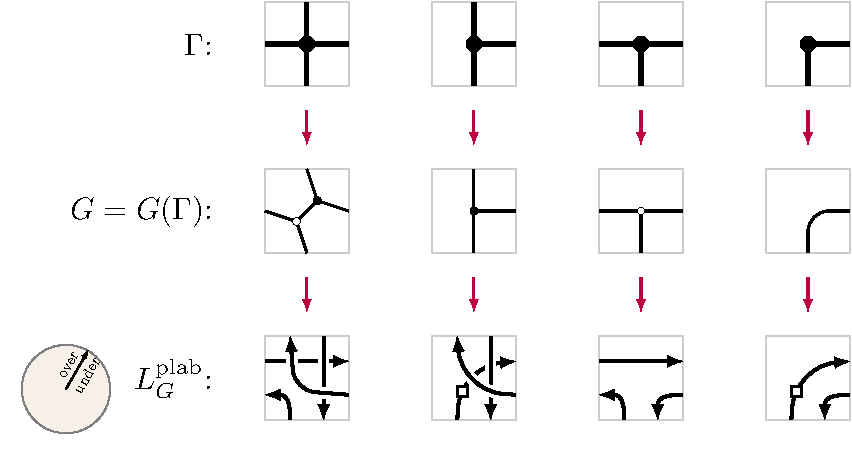
\includegraphics[width=0.7\textwidth]{../assets/838/Le_to_G.pdf}
  \caption{\label{fig:Le_to_G} Converting a Le-diagram (top row) into a plabic graph (middle row) and into a link (bottom row).}
\end{figure}



A Le-diagram $\Gamma$ can be converted into a plabic graph $G(\Gamma)$ using the local rules shown in the first two rows of \cref{fig:Le_to_G}. This plabic graph is always reduced and has strand permutation $\fp=wv^{-1}$, where $(v,w)\in\Qkn$ are recovered from $\Gamma$ using the above procedure.


%

\subsection{Properties of plabic graph links}\label{sec:plabic_links_properties}
Let $G$ be a reduced plabic graph with strand permutation $\pi=\pig$. Recall the description of the plabic graph link $\Lplab_\pi=\Lplab_G$ from \cref{sec:intro:plabic_link}. It may appear from this description that $\Lplab_G$ depends on the precise way of drawing the strands in $G$ as smooth curves, or that $\Lplab_G$ changes if one rotates the graph $G$ (since the over/under-crossings information depends on the complex arguments of the strands). However, it turns out that the link $\Lplab_G$ is in fact independent of these choices, as explained in~\cite{ACampo,STWZ,FPST}. Let us give a more invariant description of $\Lplab_G$.

Recall that $G$ is embedded in a disk $\disk:=\{x\in\C: |x|\leq 1\}$. Consider the solid torus $\disk\times S^1$, and consider an equivalence relation $\sim$ on it defined as follows: for $(x,y),(x',y')\in \disk\times S^1$, write $(x,y)\sim(x',y')$ if $x,x'\in\partial \disk$ belong to the boundary of the disk and $x=x'$. In other words, we collapse each fiber $x\times S^1$, where $x\in\partial \disk$, to a point. The resulting quotient space $\disk\times S^1/\sim$ is homeomorphic to a $3$-dimensional sphere $S^3$.

An \emph{oriented divide} is a smooth immersion of a union of oriented circles (called \emph{branches}) into $\disk$. 
 %
%
%
%
%
 Divides are required to satisfy certain genericity conditions, e.g. that any intersections between the branches must be transversal and belong to the interior of $\disk$, and that there have to be no triple intersections; see~\cite[Definitions~2.1 and~8.1]{FPST} for a complete list. 

Given a branch $\gamma$ of an oriented divide $\Divide$, we lift each point of $\gamma$ to $\disk\times S^1$ by letting the $S^1$ coordinate be the complex argument of the tangent vector of $\gamma$ at this point. By the genericity assumptions, we obtain an embedding of a union of oriented circles into $S^3$, i.e.  a link, denoted $L_\Divide$.

\begin{figure}
  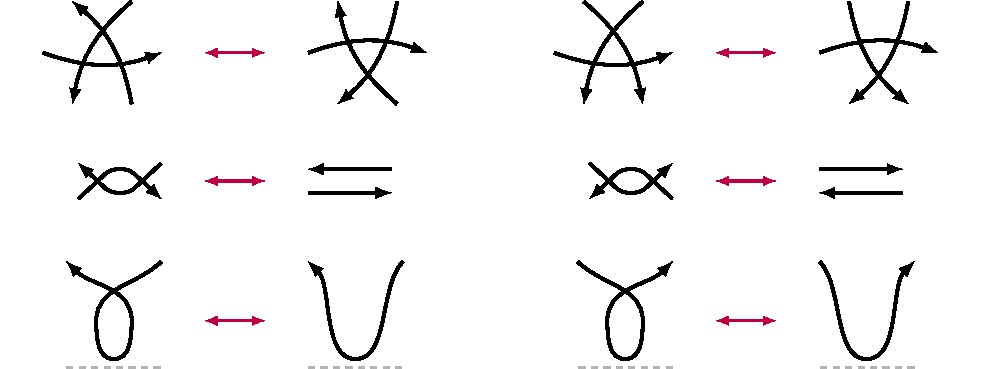
\includegraphics[width=0.7\textwidth]{../assets/838/divide_moves.pdf}
  \caption{\label{fig:divide_moves} Local moves for divides~\cite[Figures~28--30]{FPST}.}
\end{figure}


The link $L_\Divide$ is invariant under applying the local moves shown in \cref{fig:divide_moves} to $\Divide$; see~\cite[Proposition~8.4]{FPST}. We thank the anonymous referee for pointing out that the map $\Divide \mapsto L_\Divide$ coincides with the map reconstructing a Legendrian curve from its front projection. Thus, the invariance under local moves may be deduced from e.g.~\cite{Arnold}.

Take the strands in our reduced plabic graph $G$. Each of the $\n$ boundary vertices of $G$ has one incoming strand and one outgoing strand. Identifying their endpoints, we obtain an oriented divide $\Divide(G)$. It was shown in~\cite{Hirasawa} that the associated link $L_{\Divide(G)}$ is isotopic to the link $\Lplab_G$ described in \cref{sec:intro:plabic_link}. This shows that the link $\Lplab_G$ is indeed invariant under rotation of $G$ and under small perturbations of the branches of $\Divide(G)$, since this is clearly the case for $L_{\Divide(G)}$. 

\begin{remark}\label{rmk:rotation}
In what follows, it will be convenient to us to use rotational invariance of $\Lplab_G$. In our figures, we will fix some angle $\alpha\in[0,2\pi)$, and assume that the link $\Lplab_G$ is obtained by first rotating $G$ by the angle $-\alpha$, then applying the description from \cref{sec:intro:plabic_link}, and then rotating the picture back by $\alpha$. In other words, if two strands $S_1,S_2$ in $G$ intersect at some point $p$, we consider their complex arguments of tangent vectors in a different interval: $\Arg(S_1,p),\Arg(S_2,p)\in[\alpha,\alpha+2\pi)$. Then we draw $S_1$ above $S_2$ if and only if $\Arg(S_2,p)>\Arg(S_1,p)$. And then for all points $p$ where some strand $S$ satisfies $\Arg(S,p)=\alpha$, we insert line segments going to the boundary and back. In the figures, the direction $\alpha$ is indicated by the ``over/under circle'' \\
%
\centerline{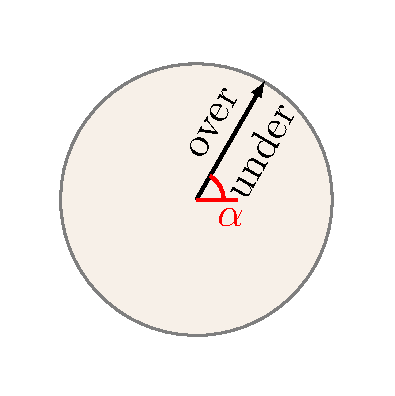
\includegraphics[width=0.17\textwidth]{../assets/838/over_under_2.pdf}}
%
and each point $p$ on a strand $S$ satisfying $\Arg(S,p)=\alpha$ is marked by $\mysq$ as in \cref{fig:over_under}.
\end{remark}






\section{Positroid link isotopies}\label{sec:positr-link-isot}
The goal of this section is to prove \cref{thm:isotopy}. We first discuss some properties of plabic graph links, and then we construct a sequence of isotopies, for any permutation $\pi\in\Sn$ without fixed points, of the links
\begin{equation*}%
\Lrich_\pi \cong  \Lplab_\pi \cong \Lperm_\pi \cong \Ltor_\pi,
\end{equation*}
in that order. When $\pi=\pi_C$ for some concave curve $C$, we will also show that
\begin{equation*}%
  \Ltor_\pi\cong\Lcox_\pi,
\end{equation*}
completing the proof.

%
%

Throughout this section, we fix a permutation $\pi\in\Sn$ without fixed points, and let $(v,w)\in\Qkn$ be the corresponding pair satisfying $\pi=wv^{-1}$,  $\Gamma$ the corresponding Le-diagram of shape $\la$, and $G$ the corresponding plabic graph, obtained from $\Gamma$ using the recipe in the first two rows of \cref{fig:Le_to_G}.

\subsection{From Richardson links to plabic graph links}\label{sec:from-rich-links}
 Our goal is to construct an isotopy between the Richardson link $\Lrich_{v,w}$ (\figref{fig:Lrich}(right)) and the plabic graph link $\Lplab_G$ (\figref{fig:Lplab}(c)).

Recall from \cref{rmk:Rich_Young} that we are drawing the Richardson braid $\beta_{v,w}=\beta(w)\cdot \beta(v)^{-1}$ in a particular way, so that the crossings of $\beta(w)$ form a shape obtained by rotating $\la$ clockwise by $135^\circ$, and the crossings of $\beta(v)^{-1}$ are drawn in some boxes of a shape obtained from the $135^\circ$-rotation of $\la$ by reflecting it along the vertical axis; see \figref{fig:Lrich}(left). Moreover, the crossings of $\beta(v)^{-1}$ are located precisely in the boxes of $\la$ which do not contain a dot in $\Gamma$. 
 %

\begin{figure}
  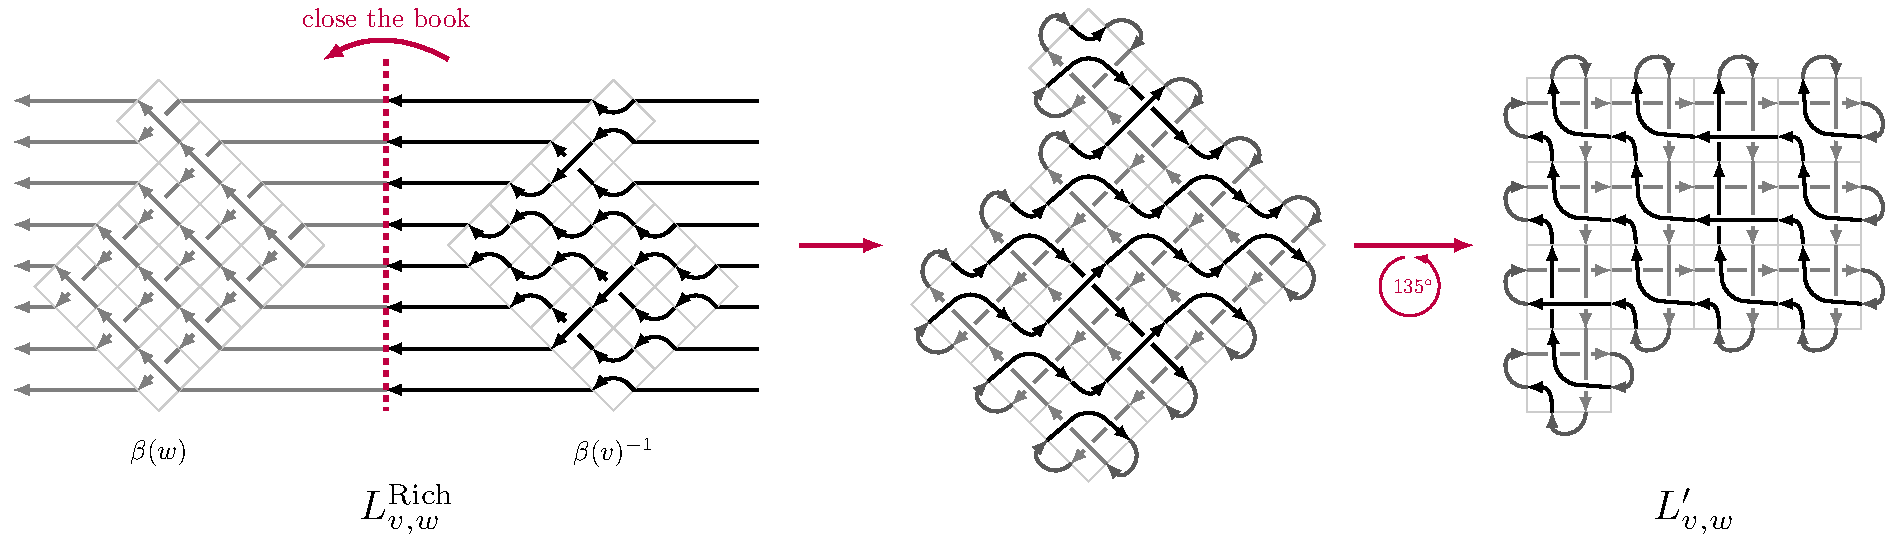
\includegraphics[width=1.0\textwidth]{../assets/838/Lrich_to_Lprime.pdf}
  \caption{\label{fig:Lrich-to-L'} Converting the link $\Lrich_{v,w}$ into $\Lrichp_{v,w}'$; see \cref{sec:from-rich-links}.}
\end{figure}


Our first goal is to draw the link $\Lrich_{v,w}$ entirely within $\la$. To do that, we take $\beta(v)^{-1}$, reflect it along the vertical axis (flipping the over/under-crossings), and place the resulting braid on top of $\beta(w)$. We rotate the result counterclockwise by $135^\circ$. Every line segment in the boundary of $\la$ contains an endpoint of a strand in $\beta(v)^{-1}$ and an endpoint of a strand in $\beta(w)$. We join these strand endpoints, obtaining a link diagram drawn inside of $\la$. This link $\Lrichp_{v,w}'$, shown in \cref{fig:Lrich-to-L'}, is clearly isotopic to $\Lrichp_{v,w}$. Intuitively, the transformation $\Lrich_{v,w}\to\Lrichp_{v,w}'$ can be described as follows: open a book, and place the left (resp. right) half of \figref{fig:Lrich}(right) onto the left (resp. right) page of the book. Then close the book with your right hand, so that the front cover of the book is at the bottom. The page containing (the reflection of) $\beta(v)^{-1}$ will be on top of the page containing $\beta(w)$. Finally, rotate the closed book $135^\circ$ counterclockwise. 


\begin{figure}
  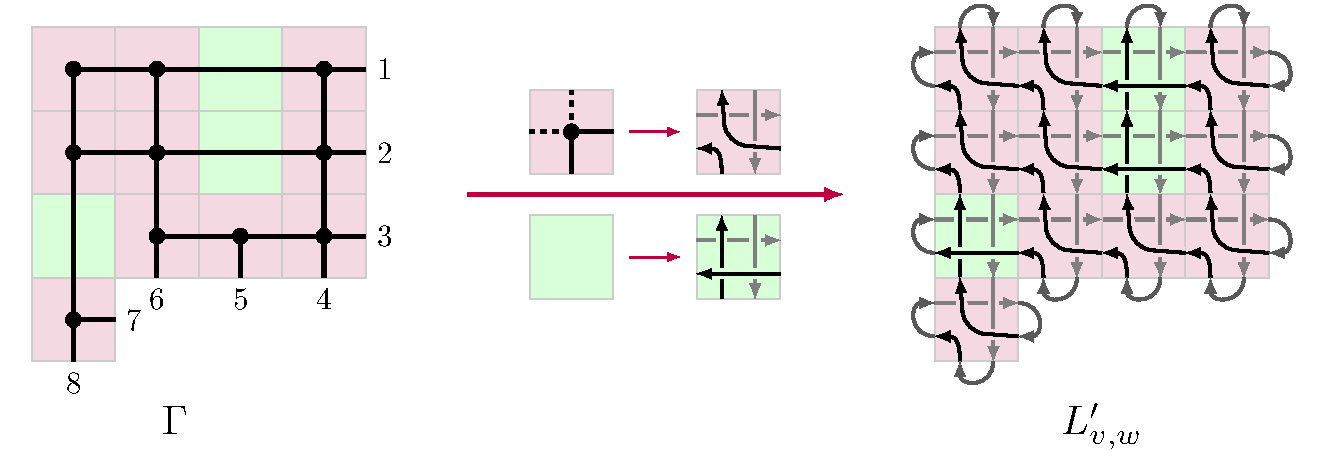
\includegraphics[width=0.9\textwidth]{../assets/838/Gamma_to_Lprime.pdf}
  \caption{\label{fig:Gamma-to-L'} Converting a Le-diagram $\Gamma$ into a link $L'_{v,w}$.}
\end{figure}




An alternative description of the link $\Lrichp_{v,w}'$ can be obtained directly from the Le-diagram $\Gamma$ by replacing each box containing a dot as shown in \figref{fig:Gamma-to-L'}(middle top) and each box not containing a dot as shown in \figref{fig:Gamma-to-L'}(middle bottom). For example, the Le-diagram in \figref{fig:Gamma-to-L'}(left) gets converted into the link $\Lrichp_{v,w}'$ in \figref{fig:Gamma-to-L'}(right); this is the same link as in \figref{fig:Lrich-to-L'}(right). Since $\pi$ has no fixed points, each row and each column of $\Gamma$ contains at least one dot. Consider some column $j$ of $\Gamma$ and let $b_j$ be the highest box in it which contains a dot. The part of $\Lrichp_{v,w}'$ above $b_j$ contains a strand going vertically to the top boundary and then back, passing between all the horizontal strands that it encounters along the way. We may therefore contract this piece of the strand to be fully contained inside $b_j$, as shown in \figref{fig:pull}(far left). Repeating this procedure for each column $j=1,2,\dots,\la_1$, we obtain a link $\Lrichp_{v,w}''$ isotopic to $\Lrichp_{v,w}'$; see \figref{fig:pull}(middle).

\begin{figure}
  \setlength{\tabcolsep}{0pt}
\begin{tabular}{c|c}
\begin{tikzpicture}[baseline=(Z.base)]
\coordinate(Z) at (0,0);
\node(A) at (0,2.05){
  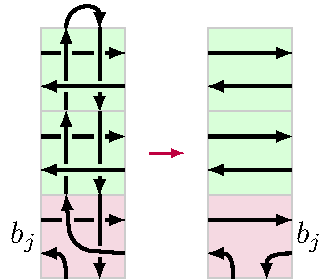
\includegraphics[width=0.2\textwidth]{../assets/838/pull.pdf}
};
\end{tikzpicture}
&
  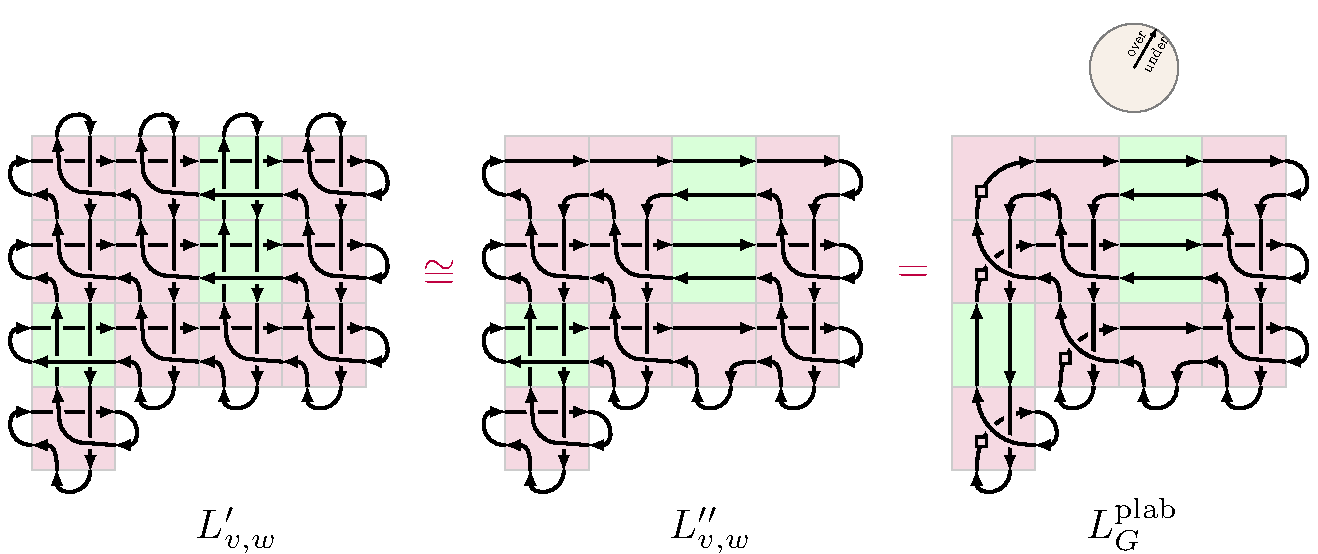
\includegraphics[width=0.78\textwidth]{../assets/838/pull_to_L.pdf}
\end{tabular}
  \caption{\label{fig:pull} An isotopy from $\Lrichp_{v,w}'$ to $\Lplab_G$.}
\end{figure}



Finally, we claim that the link $\Lrichp_{v,w}''$ is isotopic to the plabic graph link $\Lplab_G$. To see this, we choose the angle $\alpha$ from \cref{rmk:rotation} to be $80^\circ$. Then combining the rules from \cref{fig:Le_to_G} for converting the Le-diagram $\Gamma$ into the plabic graph $G$ with the description of $\Lplab_G$ given in \cref{sec:plabic_links_properties}, we see that a planar diagram of $\Lplab_G$ is obtained from $\Gamma$ via the rules shown in the last two rows of \cref{fig:Le_to_G}. Replacing each square (where $\Arg(S,p)=\alpha$) by a horizontal segment going to the left boundary above all other strands and back below all other strands, we see that $\Lplab_G= \Lrichp_{v,w}''$; see \figref{fig:pull}(far right). To summarize, we have constructed explicit isotopies
\begin{equation*}%
  \Lrich_\pi=\Lrich_{v,w}\cong\Lrichp_{v,w}'\cong\Lrichp_{v,w}''=\Lplab_G.
\end{equation*}



\begin{figure}
  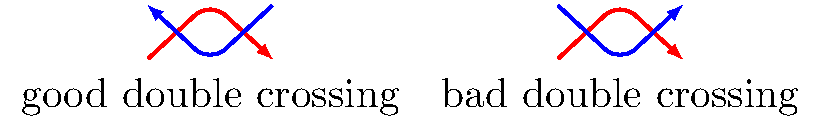
\includegraphics[width=0.5\textwidth]{../assets/838/double.pdf}
  \caption{\label{fig:double} Good and bad double crossings of strands in plabic graphs.}
\end{figure}


\subsection{From plabic graph links to permutation links}
Our goal is to find an isotopy $\Lplab_\pi\cong \Lperm_\pi$. Let $G$ be a reduced plabic graph with strand permutation $\pi$. Let $\Divide=\Divide(G)$ be the oriented divide obtained from $G$ as in \cref{sec:plabic_links_properties}. Let $1,2,\dots,\n$ be the boundary vertices of $G$. Since $G$ is reduced, it contains no bad double crossings shown in \figref{fig:double}(right). Thus, it is clear that applying the moves from \cref{fig:divide_moves}, one can transform $\Divide$ into an oriented divide $\Divide'$ obtained by drawing a straight arrow $i\to \pi(i)$ for each $i\in[\n]$. The moves from \cref{fig:divide_moves} give rise to link isotopies, so $L_\Divide\cong L_{\Divide'}$. Let us move the boundary vertices $1,2,\dots,\n$ smoothly to the points $1',2',\dots,\n'$ which are located clockwise on the left semicircle of $\partial \disk$, i.e.  on the subset of $\partial\disk$ with negative real part. Let $\Divide''$ be the oriented divide obtained by drawing a straight arrow $i'\to \pi(i)'$ for each $i\in[\n]$. It follows that $L_{\Divide'}\cong L_{\Divide''}$.
%
 Let $i,j\in[\n]$ be such that the corresponding arrows $S_i:=(i'\to \pi(i)')$ and $S_j:=(j'\to \pi(j)')$ of $\Divide''$ cross at some point $p$. Consider the arguments of the tangent vectors $0\leq \Arg(S_i,p)\neq\Arg(S_j,p)<2\pi$. Then it is easy to check that $\Arg(S_i,p)>\Arg(S_j,p)$ if and only if $\pi(i)<\pi(j)$. 
%
 Comparing to the description in \cref{sec:intro:perm_links}, we get that $L_{\Divide''}\cong\Lperm_\pi$.



\subsection{From permutation links to toric permutation links}\label{sec:perm-to-toric}
Our goal is to find an isotopy $\Lperm_\pi\cong\Ltor_\pi$. Recall from \cref{rmk:grid} that $\Ltor_\pi$ is isotopic to the \emph{planar grid link} denoted $\Lgrid_\pi$; see \figref{fig:grid_iso}(a--c). In $\Lgridt_\pi$ and $\Lgrid_\pi$, the vertical arrows are drawn above the horizontal arrows. 

The main diagonal $y=1-x$ of the square $[0,1]^2$ divides $\Lgrid_\pi$ into the \emph{lower-triangular} and the \emph{upper-triangular} parts. In the lower-triangular part, all vertical arrows point down and all horizontal arrows point right, while in the upper-triangular part, all vertical arrows point up and all horizontal arrows point left. 
Let us take the lower-triangular part and reflect it around the main diagonal, placing it below the upper-triangular part; see \figref{fig:grid_iso}(c--d). We obtain a planar diagram of a link which we denote $L_\pi'$. Clearly, $L_\pi'\cong \Lgrid_\pi$. The diagram of $L_\pi'$ contains arrows pointing, up, left, down, and right. It follows that the over/under-crossings rule  in $L_\pi'$ is given by the following total order on the arrow directions: up $>$ left $>$ down $>$ right. In particular, $L_\pi'$ is a divide link for the angle $\alpha=45^\circ$ from \cref{rmk:rotation} (where the main diagonal is treated as part of the boundary of the disk), and we get that $L_\pi'\cong\Lperm_\pi$. 
%

\subsection{From toric permutation links to Coxeter links}\label{sec:tor_to_Cox}
First, we introduce a more general class of links, associated to arbitrary monotone curves inside the $k\times(\n-k)$ rectangle.

%
%
We say that $C_g$ is a \emph{monotone curve} if it is the plot of a strictly monotone increasing function $g(x):[0,\n-k]\to[0,k]$ satisfying $g(0)=0$, $g(\n-k)=k$, and $g(j)\notin\Z$ for all $j=1,2,\dots,\n-k-1$. Thus, the curve $C_g$ passes through the points $(0,0)$ and $(\n-k,k)$, but through no other lattice points. To any monotone curve $C_g$ we associate a link $L_g$ drawn on the surface of $\T$. The planar diagram of $L_g$ is obtained from the projection $\Cproj_g$ of $C_g$ to $\T$ via the following rule: whenever  two points $(x,g(x))$, $(x',g(x'))$ on $C_g$ (with $x<x'$) project to the same point of $\Cproj_g$, we draw the projection of $(x,g(x))$ above the projection of $(x',g(x'))$. 

The link diagram of $L_g$ is drawn on the torus $\T$, and therefore it is natural to think of $L_g$ itself as a link inside the \emph{thickened torus} $\T\times[0,1]$. Given a point $p=(x,g(x))\in C_g$, we denote by $\projtx p\in \T$ the projection of $p$ to $\T$, and we let $\left(\projtx p,1-\frac{x}{\n-k}\right)$ be the corresponding point in $\T\times[0,1]$. This yields an embedding of $C_g$ into $\T\times[0,1]$. Under this embedding, the points $(0,0)$ and $(\n-k,k)$ map to $((0,0),1)$ and $((0,0),0)$, respectively. Adding a line segment connecting $((0,0),1)$ to $((0,0),0)$, we obtain a representation of the link $L_g$ inside $\T\times[0,1]$. An obvious consequence of this construction is that the link $L_g$ only depends on the set of lattice points below the plot of $g$.
\begin{corollary} \label{cor:monotone_curves}
Let $C_g$, $C_h$ be two monotone curves, and assume that for each $j=1,2,\dots,\n-k-1$, we have $\lfloor g(j)\rfloor=\lfloor h(j)\rfloor$. Then the links $L_g$ and $L_h$ are isotopic. 
\end{corollary}

Suppose now that $\pi=\pi_C$ for a concave curve $C$. Our goal is to find an isotopy $\Ltor_\pi\cong\Lcox_C$. Comparing the above description to the one in \cref{sec:intro:cox_link}, we see that when $g$ is the concave down function satisfying $C=C_g$, we have $\Ltor_\pi\cong L_g$. Our goal is to choose a monotone curve $C_h$ such that $L_g\cong L_h$ by \cref{cor:monotone_curves}, and such that $L_h\cong \Lcox_C$. 
 %

\begin{figure}
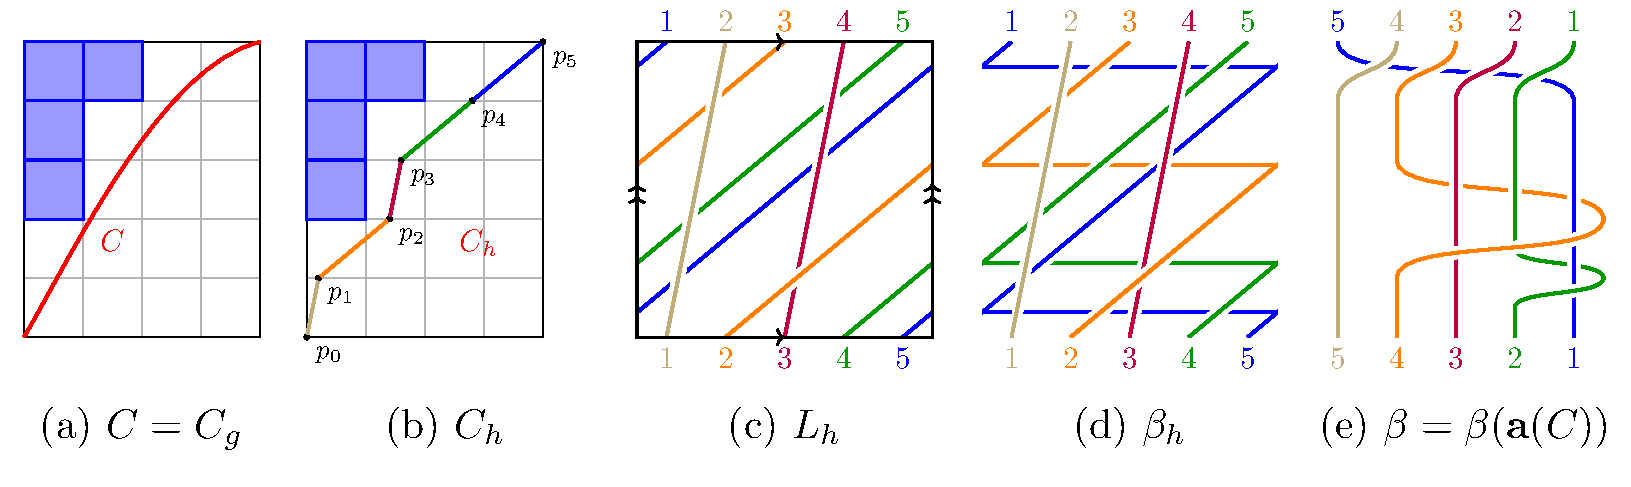
\includegraphics[width=1.0\textwidth]{../assets/838/C_to_beta.pdf}
  \caption{\label{fig:C_to_beta} Converting a concave curve $C$ into the Coxeter link $\beta(\abf(C))$; see \cref{sec:tor_to_Cox}.}
\end{figure}


Let $\la=\la_C=(\la_1\geq \la_2\geq\dots\geq \la_k=0)$ be the Young diagram above $C$. For $r=0,1,\dots,k-1$, let $p_r:= \left(\la_{k-r}+\frac rk,r\right)$. Thus, $p_0=(0,0)$. Let $p_{k}:=(\n-k,k)$. Let $h$ be the piecewise-linear function whose plot passes through the points $p_0,p_1,\dots,p_k$, and let $C_h$ be the corresponding monotone curve; see \figref{fig:C_to_beta}(b). Indeed, by \cref{cor:monotone_curves}, we have $L_g\cong L_h$. It remains to establish the isotopy $L_h\cong \Lcox_C$. 

Let $\beta=\beta(\abf(C))$ be the Coxeter braid associated to $C$, defined in~\eqref{eq:beta_abf_dfn}. It is a braid on $k$ strands. For $i=1,2,\dots,k$, let $S_i(\beta)$ be the strand of $\beta$ whose left endpoint is labeled by~$i$. Thus, the right endpoint of $S_i(\beta)$ is labeled by $i+1$ for $i<k$ and by $1$ for $i=k$. On the other hand, the link diagram of $L_h$ in $\T$ intersects the line $y=0$ in exactly $k$ points with horizontal coordinates $\frac rk$ for $r=0,1,\dots, k-1$. We would like to view $L_h$ as the closure of a $k$-strand braid $\beta_h$ in the solid torus; see \figref{fig:C_to_beta}(c--d). The braid $\beta_h$ is obtained from $L_h$ via the following procedure: whenever a strand of $L_h$ passes through some point $(1,y)\in[0,1]^2$ and continues from the point $(0,y)\in[0,1]^2$, we connect the points $(0,y)$ and $(1,y)$ by a horizontal line segment that is drawn below all strands of $L_h$. The result is a drawing of a braid connecting $k$ points at the bottom of $[0,1]^2$ to $k$ points at the top of $[0,1]^2$. 

For $i=1,2,\dots, k-1$, let $S_i(\beta_h)$ be the piece of $\beta_h$ connecting the point $(\frac{i-1}k,0)$ to the point $(\frac ik,1)$. For $i=k$, let $S_k(\beta_h)$ be the remaining piece of $\beta_h$, connecting $(\frac{k-1}k,0)$ to $(0,1)$. See \figref{fig:C_to_beta}(d--e).

We claim that the braids $\beta_h$ and $\beta$ are isotopic. We compare them strand-by-strand, identifying $S_i(\beta)$ with $S_{k+1-i}(\beta_h)$ for $i=1,2,\dots,k$, in that order. (This correspondence is indicated via colors in \figref{fig:C_to_beta}(d--e).) For convenience, we rotate the drawing of $\beta$ by $90^\circ$ counterclockwise. The strand $S_1(\beta)$ moves straight up during the $\ell_2^{a_2}\cdots \ell_k^{a_k}$ part, and then it moves left under all other strands. We apply an isotopy to make $S_k(\beta_h)$ move straight up towards the top boundary of $[0,1]^2$, and then move left under all other strands. Recall that we have a sequence $\abf(C)=(a_2,\dots,a_k)$ given by $a_i=\la_{i-1}-\la_i$ for $i=2,\dots,k$. Thus, the strand $S_2(\beta)$ wraps around $S_1(\beta)$ exactly $a_2$ times. On the other hand, $S_{k-1}(\beta_h)$ is the projection to $\T$ of the line segment of $C_h$ connecting $p_{k-1}$ to $p_k$. This projection intersects the vertical boundary of $\T$ exactly $a_2$ times. Therefore $S_{k-1}(\beta_h)$ wraps around $S_k(\beta_h)$ exactly $a_2$ times. Continuing in this fashion, we see that for $i=3,\dots,k$, the strand $S_i(\beta)$ wraps around the union $S_1(\beta)\cup S_2(\beta)\cup\dots\cup S_{i-1}(\beta)$ exactly $a_i$ times. On the other hand, the strand $S_{k+1-i}(\beta_h)$ wraps around the union $S_k(\beta_h)\cup S_{k-1}(\beta)\cup\dots\cup S_{k+2-i}$ exactly $a_i$ times. This shows that the braids $\beta$ and $\beta_h$ are isotopic, and therefore we get an isotopy $\Lcox_C\cong L_h$ between their closures.

\begin{remark}
The above construction is extended to links with multiple components (resp. to monotone curves passing through some lattice points in the interior of the rectangle) in~\cite[Section~7.3]{GL_EHA}.
\end{remark} 


\begin{thebibliography}{MMMMMM}
\bibitem[1]{ACampo} A’Campo, Norbert Real deformations and complex topology of plane curve singularities, Ann. Fac. Sci. Toulouse Math. (6), Volume 8 (1999) no. 1, pp. 5-23 \href{https://alco.centre-mersenne.org/articles/10.5802/alco.345/#ACampo}{Publisher reference}.
\bibitem[2]{ALS} Arkani-Hamed, Nima; Lam, Thomas; Spradlin, Marcus Positive configuration space, Comm. Math. Phys., Volume 384 (2021) no. 2, pp. 909-954 \href{https://alco.centre-mersenne.org/articles/10.5802/alco.345/#ALS}{Publisher reference}.
\bibitem[3]{Arnold} Arnol’d, V. I. The geometry of spherical curves and quaternion algebra, Uspekhi Mat. Nauk, Volume 50 (1995) no. 1(301), pp. 3-68 \href{https://alco.centre-mersenne.org/articles/10.5802/alco.345/#Arnold}{Publisher reference}.
\bibitem[4]{BMS} Bazier-Matte, Véronique; Schiffler, Ralf Knot theory and cluster algebras, Adv. Math., Volume 408 (2022), Paper no. 108609, 45 pages \href{https://alco.centre-mersenne.org/articles/10.5802/alco.345/#BMS}{Publisher reference}.
\bibitem[5]{BHMPS} Blasiak, Jonah; Haiman, Mark; Morse, Jennifer; Pun, Anna; Seelinger, George H. A shuffle theorem for paths under any line, Forum Math. Pi, Volume 11 (2023), Paper no. e5, 38 pages \href{https://alco.centre-mersenne.org/articles/10.5802/alco.345/#BHMPS}{Publisher reference}.
\bibitem[6]{BuSc} Burban, Igor; Schiffmann, Olivier On the Hall algebra of an elliptic curve, I, Duke Math. J., Volume 161 (2012) no. 7, pp. 1171-1231 \href{https://alco.centre-mersenne.org/articles/10.5802/alco.345/#BuSc}{Publisher reference}.
\bibitem[7]{CG} Casals, Roger; Gao, Honghao Infinitely many Lagrangian fillings, Ann. of Math. (2), Volume 195 (2022) no. 1, pp. 207-249 \href{https://alco.centre-mersenne.org/articles/10.5802/alco.345/#CG}{Publisher reference}.
\bibitem[8]{CGGLSS} Casals, Roger; Gorsky, Eugene; Gorsky, Mikhail; Le, Ian; Shen, Linhui; Simental, José Cluster structures on braid varieties, 2022 \href{https://alco.centre-mersenne.org/articles/10.5802/alco.345/#CGGLSS}{Publisher reference}.
\bibitem[9]{CGGS} Casals, Roger; Gorsky, Eugene; Gorsky, Mikhail; Simental, José Positroid Links and Braid varieties, 2024 \href{https://alco.centre-mersenne.org/articles/10.5802/alco.345/#CGGS}{Publisher reference}.
\bibitem[10]{CW} Casals, Roger; Weng, Daping Microlocal theory of Legendrian links and cluster algebras, Geom. Topol., Volume 28 (2024) no. 2, pp. 901-1000 \href{https://alco.centre-mersenne.org/articles/10.5802/alco.345/#CW}{Publisher reference}.
\bibitem[11]{Deodhar} Deodhar, Vinay V. On some geometric aspects of Bruhat orderings. I. A finer decomposition of Bruhat cells, Invent. Math., Volume 79 (1985) no. 3, pp. 499-511 \href{https://alco.centre-mersenne.org/articles/10.5802/alco.345/#Deodhar}{Publisher reference}.
\bibitem[12]{FPST} Fomin, Sergey; Pylyavskyy, Pavlo; Shustin, Eugenii; Thurston, Dylan Morsifications and mutations, J. Lond. Math. Soc. (2), Volume 105 (2022) no. 4, pp. 2478-2554 \href{https://alco.centre-mersenne.org/articles/10.5802/alco.345/#FPST}{Publisher reference}.
\bibitem[13]{FWZ_book} Fomin, Sergey; Williams, Lauren; Zelevinsky, Andrei Introduction to Cluster Algebras. Chapters 1-3, 2021 \href{https://alco.centre-mersenne.org/articles/10.5802/alco.345/#FWZ_book}{Publisher reference}.
\bibitem[14]{FZ} Fomin, Sergey; Zelevinsky, Andrei Cluster algebras. I. Foundations, J. Amer. Math. Soc., Volume 15 (2002) no. 2, pp. 497-529 \href{https://alco.centre-mersenne.org/articles/10.5802/alco.345/#FZ}{Publisher reference}.
\bibitem[15]{HOMFLY} Freyd, P.; Yetter, D.; Hoste, J.; Lickorish, W. B. R.; Millett, K.; Ocneanu, A. A new polynomial invariant of knots and links, Bull. Amer. Math. Soc. (N.S.), Volume 12 (1985) no. 2, pp. 239-246 \href{https://alco.centre-mersenne.org/articles/10.5802/alco.345/#HOMFLY}{Publisher reference}.
\bibitem[16]{GL_cat_combin} Galashin, Pavel; Lam, Thomas Positroid Catalan numbers, 2021 \href{https://alco.centre-mersenne.org/articles/10.5802/alco.345/#GL_cat_combin}{Publisher reference}.
\bibitem[17]{GL_qtcat} Galashin, Pavel; Lam, Thomas Positroids, knots, and q,t-Catalan numbers, Sém. Lothar. Combin., Volume 85B (2021), Paper no. 54, 12 pages \href{https://alco.centre-mersenne.org/articles/10.5802/alco.345/#GL_qtcat}{Publisher reference}.
\bibitem[18]{GL_EHA} Galashin, Pavel; Lam, Thomas Monotone links in DAHA and EHA, 2023 \href{https://alco.centre-mersenne.org/articles/10.5802/alco.345/#GL_EHA}{Publisher reference}.
\bibitem[19]{GL_cluster} Galashin, Pavel; Lam, Thomas Positroid varieties and cluster algebras, Ann. Sci. Éc. Norm. Supér. (4), Volume 56 (2023) no. 3, pp. 859-884 \href{https://alco.centre-mersenne.org/articles/10.5802/alco.345/#GL_cluster}{Publisher reference}.
\bibitem[20]{GLSBS2} Galashin, Pavel; Lam, Thomas; Sherman-Bennett, Melissa Braid variety cluster structures, II: general type, 2023 \href{https://alco.centre-mersenne.org/articles/10.5802/alco.345/#GLSBS2}{Publisher reference}.
\bibitem[21]{GLSBS1} Galashin, Pavel; Lam, Thomas; Sherman-Bennett, Melissa; Speyer, David Braid variety cluster structures, I: 3D plabic graphs, 2022 \href{https://alco.centre-mersenne.org/articles/10.5802/alco.345/#GLSBS1}{Publisher reference}.
\bibitem[22]{GePf} Geck, Meinolf; Pfeiffer, Götz On the irreducible characters of Hecke algebras, Adv. Math., Volume 102 (1993) no. 1, pp. 79-94 \href{https://alco.centre-mersenne.org/articles/10.5802/alco.345/#GePf}{Publisher reference}.
\bibitem[23]{GN} Gorsky, Eugene; Neguţ, Andrei Refined knot invariants and Hilbert schemes, J. Math. Pures Appl. (9), Volume 104 (2015) no. 3, pp. 403-435 \href{https://alco.centre-mersenne.org/articles/10.5802/alco.345/#GN}{Publisher reference}.
\bibitem[24]{GNR} Gorsky, Eugene; Neguţ, Andrei; Rasmussen, Jacob Flag Hilbert schemes, colored projectors and Khovanov-Rozansky homology, Adv. Math., Volume 378 (2021), Paper no. 107542, 115 pages \href{https://alco.centre-mersenne.org/articles/10.5802/alco.345/#GNR}{Publisher reference}.
\bibitem[25]{HiIn} Hikami, Kazuhiro; Inoue, Rei Braids, complex volume and cluster algebras, Algebr. Geom. Topol., Volume 15 (2015) no. 4, pp. 2175-2194 \href{https://alco.centre-mersenne.org/articles/10.5802/alco.345/#HiIn}{Publisher reference}.
\bibitem[26]{Hirasawa} Hirasawa, Mikami Visualization of A’Campo’s fibered links and unknotting operation, Topology Appl., Volume 121 (2002) no. 1, pp. 287-304 \href{https://alco.centre-mersenne.org/articles/10.5802/alco.345/#Hirasawa}{Publisher reference}.
\bibitem[27]{KAT} The Knot Atlas: The Thistlethwaite Link Table \url{http://katlas.org/wiki/The_Thistlethwaite_Link_Table} \href{https://alco.centre-mersenne.org/articles/10.5802/alco.345/#KAT}{Publisher reference}.
\bibitem[28]{KAT_knot} The Knot Atlas: The Rolfsen Knot Table \url{http://katlas.org/wiki/The_Rolfsen_Knot_Table} \href{https://alco.centre-mersenne.org/articles/10.5802/alco.345/#KAT_knot}{Publisher reference}.
\bibitem[29]{KhoSoe} Khovanov, Mikhail Triply-graded link homology and Hochschild homology of Soergel bimodules, Internat. J. Math., Volume 18 (2007) no. 8, pp. 869-885 \href{https://alco.centre-mersenne.org/articles/10.5802/alco.345/#KhoSoe}{Publisher reference}.
\bibitem[30]{KR1} Khovanov, Mikhail; Rozansky, Lev Matrix factorizations and link homology, Fund. Math., Volume 199 (2008) no. 1, pp. 1-91 \href{https://alco.centre-mersenne.org/articles/10.5802/alco.345/#KR1}{Publisher reference}.
\bibitem[31]{KR2} Khovanov, Mikhail; Rozansky, Lev Matrix factorizations and link homology. II, Geom. Topol., Volume 12 (2008) no. 3, pp. 1387-1425 \href{https://alco.centre-mersenne.org/articles/10.5802/alco.345/#KR2}{Publisher reference}.
\bibitem[32]{KLS} Knutson, Allen; Lam, Thomas; Speyer, David E Positroid varieties: juggling and geometry, Compos. Math., Volume 149 (2013) no. 10, pp. 1710-1752 \href{https://alco.centre-mersenne.org/articles/10.5802/alco.345/#KLS}{Publisher reference}.
\bibitem[33]{LamCDM} Lam, Thomas Totally nonnegative Grassmannian and Grassmann polytopes, Current developments in mathematics 2014, Int. Press, Somerville, MA, 2016, pp. 51-152 \href{https://alco.centre-mersenne.org/articles/10.5802/alco.345/#LamCDM}{Publisher reference}.
\bibitem[34]{LS} Lam, Thomas; Speyer, David E Cohomology of cluster varieties I: Locally acyclic case, Algebra Number Theory, Volume 16 (2022) no. 1, pp. 179-230 \href{https://alco.centre-mersenne.org/articles/10.5802/alco.345/#LS}{Publisher reference}.
\bibitem[35]{LS2} Lam, Thomas; Speyer, David E Cohomology of cluster varieties II: Acyclic case, J. Lond. Math. Soc. (2), Volume 108 (2023) no. 6, pp. 2377-2414 \href{https://alco.centre-mersenne.org/articles/10.5802/alco.345/#LS2}{Publisher reference}.
\bibitem[36]{Lec} Leclerc, B. Cluster structures on strata of flag varieties, Adv. Math., Volume 300 (2016), pp. 190-228 \href{https://alco.centre-mersenne.org/articles/10.5802/alco.345/#Lec}{Publisher reference}.
\bibitem[37]{LeeSch} Lee, Kyungyong; Schiffler, Ralf Cluster algebras and Jones polynomials, Selecta Math. (N.S.), Volume 25 (2019) no. 4, Paper no. 58, 41 pages \href{https://alco.centre-mersenne.org/articles/10.5802/alco.345/#LeeSch}{Publisher reference}.
\bibitem[38]{Lickorish} Lickorish, W. B. Raymond An introduction to knot theory, Graduate Texts in Mathematics, 175, Springer-Verlag, New York, 1997, x+201 pages \href{https://alco.centre-mersenne.org/articles/10.5802/alco.345/#Lickorish}{Publisher reference}.
\bibitem[39]{knotinfo} Livingston, Charles; Moore, Allison H. KnotInfo: Table of Knot Invariants, 2022 \href{https://alco.centre-mersenne.org/articles/10.5802/alco.345/#knotinfo}{Publisher reference}.
\bibitem[40]{Mellit_Cell} Mellit, Anton Cell decompositions of character varieties, 2019 \href{https://alco.centre-mersenne.org/articles/10.5802/alco.345/#Mellit_Cell}{Publisher reference}.
\bibitem[41]{Muller} Muller, Greg Locally acyclic cluster algebras, Adv. Math., Volume 233 (2013), pp. 207-247 \href{https://alco.centre-mersenne.org/articles/10.5802/alco.345/#Muller}{Publisher reference}.
\bibitem[42]{Muller_skein} Muller, Greg Skein and cluster algebras of marked surfaces, Quantum Topol., Volume 7 (2016) no. 3, pp. 435-503 \href{https://alco.centre-mersenne.org/articles/10.5802/alco.345/#Muller_skein}{Publisher reference}.
\bibitem[43]{MSLA} Muller, Greg; Speyer, David E Cluster algebras of Grassmannians are locally acyclic, Proc. Amer. Math. Soc., Volume 144 (2016) no. 8, pp. 3267-3281 \href{https://alco.centre-mersenne.org/articles/10.5802/alco.345/#MSLA}{Publisher reference}.
\bibitem[44]{ObRo} Oblomkov, A.; Rozansky, L. Homfly-PT homology of Coxeter links, Transform. Groups, Volume 28 (2023) no. 3, pp. 1245-1275 \href{https://alco.centre-mersenne.org/articles/10.5802/alco.345/#ObRo}{Publisher reference}.
\bibitem[45]{OSS} Ozsváth, Peter S.; Stipsicz, András I.; Szabó, Zoltán Grid homology for knots and links, Mathematical Surveys and Monographs, 208, American Mathematical Society, Providence, RI, 2015, x+410 pages \href{https://alco.centre-mersenne.org/articles/10.5802/alco.345/#OSS}{Publisher reference}.
\bibitem[46]{Pos} Postnikov, Alexander Total positivity, Grassmannians, and networks (2006) \href{https://alco.centre-mersenne.org/articles/10.5802/alco.345/#Pos}{Publisher reference}.
\bibitem[47]{PT} Przytycki, Józef H.; Traczyk, Pawel Conway algebras and skein equivalence of links, Proc. Amer. Math. Soc., Volume 100 (1987) no. 4, pp. 744-748 \href{https://alco.centre-mersenne.org/articles/10.5802/alco.345/#PT}{Publisher reference}.
\bibitem[48]{Rolfsen} Rolfsen, Dale Knots and links, Mathematics Lecture Series, 7, Publish or Perish, Inc., Houston, TX, 1990, xiv+439 pages \href{https://alco.centre-mersenne.org/articles/10.5802/alco.345/#Rolfsen}{Publisher reference}.
\bibitem[49]{Ruth} Rutherford, Dan Thurston-Bennequin number, Kauffman polynomial, and ruling invariants of a Legendrian link: the Fuchs conjecture and beyond, Int. Math. Res. Not. (2006), Paper no. 78591, 15 pages \href{https://alco.centre-mersenne.org/articles/10.5802/alco.345/#Ruth}{Publisher reference}.
\bibitem[50]{ScVa} Schiffmann, Olivier; Vasserot, Eric The elliptic Hall algebra and the K-theory of the Hilbert scheme of 𝔸 2 , Duke Math. J., Volume 162 (2013) no. 2, pp. 279-366 \href{https://alco.centre-mersenne.org/articles/10.5802/alco.345/#ScVa}{Publisher reference}.
\bibitem[51]{Scott} Scott, J. S. Grassmannians and cluster algebras, Proc. London Math. Soc. (3), Volume 92 (2006) no. 2, pp. 345-380 \href{https://alco.centre-mersenne.org/articles/10.5802/alco.345/#Scott}{Publisher reference}.
\bibitem[52]{SSBW} Serhiyenko, K.; Sherman-Bennett, M.; Williams, L. Cluster structures in Schubert varieties in the Grassmannian, Proc. Lond. Math. Soc. (3), Volume 119 (2019) no. 6, pp. 1694-1744 \href{https://alco.centre-mersenne.org/articles/10.5802/alco.345/#SSBW}{Publisher reference}.
\bibitem[53]{SW} Shen, Linhui; Weng, Daping Cluster structures on double Bott-Samelson cells, Forum Math. Sigma, Volume 9 (2021), Paper no. e66, 89 pages \href{https://alco.centre-mersenne.org/articles/10.5802/alco.345/#SW}{Publisher reference}.
\bibitem[54]{STWZ} Shende, Vivek; Treumann, David; Williams, Harold; Zaslow, Eric Cluster varieties from Legendrian knots, Duke Math. J., Volume 168 (2019) no. 15, pp. 2801-2871 \href{https://alco.centre-mersenne.org/articles/10.5802/alco.345/#STWZ}{Publisher reference}.
\bibitem[55]{STZ} Shende, Vivek; Treumann, David; Zaslow, Eric Legendrian knots and constructible sheaves, Invent. Math., Volume 207 (2017) no. 3, pp. 1031-1133 \href{https://alco.centre-mersenne.org/articles/10.5802/alco.345/#STZ}{Publisher reference}.
\bibitem[56]{Trinh} Trinh, Minh-Tâm Quang From the Hecke Category to the Unipotent Locus, 2021 \href{https://alco.centre-mersenne.org/articles/10.5802/alco.345/#Trinh}{Publisher reference}.
\bibitem[57]{Turaev} Turaev, V. G. The Conway and Kauffman modules of a solid torus, Zap. Nauchn. Sem. Leningrad. Otdel. Mat. Inst. Steklov. (LOMI), Volume 167 (1988) no. 6, p. 79-89, 190 \href{https://alco.centre-mersenne.org/articles/10.5802/alco.345/#Turaev}{Publisher reference}.
\end{thebibliography}
\end{document}
